\documentclass[aspectratio=169]{beamer}
\usepackage[utf8]{inputenc}
\usepackage{hyperref}
\usepackage{amsmath,amsfonts,amsthm,bm}
\usepackage{color}
\usepackage{graphicx} % Allows including images
\usepackage{subcaption}
\usepackage{booktabs} % Allows the use of \toprule, \midrule and \bottomrule in tables
\usepackage{tikz}
\usetikzlibrary{automata,positioning,shapes.geometric,shapes.misc,arrows}
%\usepackage{pgfplots}
\usepackage{listings}
\usepackage{courier}
\usepackage[version=4]{mhchem}
\usepackage{array}

\lstset{ %
    basicstyle=\scriptsize\ttfamily, % fonts that are used for the code
    breakatwhitespace=false,         % sets if automatic breaks should only happen at whitespace
%breaklines=true,                 % sets automatic line breaking
%captionpos=b,                    % sets the caption-position to bottom
    commentstyle=\color{gray}\textit,    % comment style
    keepspaces=true,                 % keeps spaces in text, useful for keeping indentation of code (possibly needs columns=flexible)
    keywordstyle=\color{blue},       % keyword style
    language=Python,                 % the language of the code
%otherkeywords={*,...},          % if you want to add more keywords to the set
    rulecolor=\color{black},         % if not set, the frame-color may be changed on line-breaks within not-black text (e.g. comments (green here))
    showspaces=false,                % show spaces everywhere adding particular underscores; it overrides 'showstringspaces'
    showstringspaces=false,          % underline spaces within strings only
    showtabs=false,                  % show tabs within strings adding particular underscores
    stringstyle=\color{red}, % string literal style
    tabsize=4,                       % sets default tabsize to 2 spaces
    columns=fixed                    % Using fixed column width (for e.g. nice alignment)
}

\hypersetup{
    colorlinks=true,
    linkcolor=red,
    filecolor=magenta,
    urlcolor=red,
}

\DeclareMathOperator*{\argmax}{argmax}
\DeclareMathOperator*{\argmin}{argmin}
\let \vec \mathbf

\newcommand{\classname}{NANO266}
\newcommand{\classyear}{Fall 2024}
\mode<presentation> {
    \usetheme{CambridgeUS}
    \setbeamertemplate{footline}[text line]{%
        \parbox{\linewidth}{\vspace*{-8pt}\classname\hfill\classyear\hfill\insertpagenumber}}

    %\setbeamertemplate{footline}[page number]
    \setbeamertemplate{navigation symbols}{}
}


\title[\classname Properties of Periodic Solids from QM]{\classname~- Quantum Mechanical Modeling of Materials and Nanostructures\\Properties of Periodic Solids from QM}

\author{Shyue Ping Ong}
\institute[UCSD]{University of California, San Diego\\
\medskip
}
\date{\classyear} % Date, can be changed to a custom date

\begin{document}


    \begin{frame}
        \titlepage % Print the title page as the first slide
    \end{frame}

    \begin{frame}{Typical Calculation Workflow}
        \begin{figure}
            \centering
            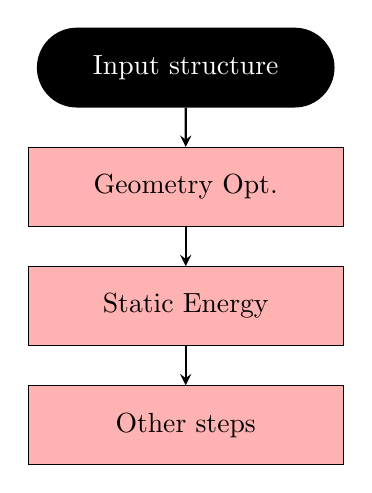
\begin{tikzpicture}[node distance=0.5cm]
                \tikzstyle{io} = [rounded rectangle, minimum width=4cm, minimum height=1cm,text centered, draw=black, fill=black, text=white]
                \tikzstyle{process} = [rectangle, minimum width=4cm, minimum height=1cm,text centered, draw=black, fill=red!30]
                \tikzstyle{decision} = [diamond,
                draw = purple,
                text = red,
                fill = pink!50,
                minimum width = 2.5cm,
                minimum height = 3cm]
                \tikzstyle{arrow} = [thick,->,>=stealth]
                \node (node1) [io, draw] {Input structure};
                \node (node2) [process, below=of node1] {Geometry Opt.};
                \node (node3) [process, below=of node2] {Static Energy};
                \node (node4) [process, below=of node3] {Other steps};

                \draw [arrow] (node1) -- (node2);
                \draw [arrow] (node2) -- (node3);
                \draw [arrow] (node3) -- (node4);
            \end{tikzpicture}
        \end{figure}

    \end{frame}

    \begin{frame}{Geometry Optimization}
        Otherwise know as ``relaxing the structure''\newline
        \newline
        Typical options in geometry optimization
        \begin{itemize}
            \item Full: cell shape, size and position of atoms are allowed to change.
            \item Fixed cell shape and size: Only position of atoms are allowed to change. E.g., defect calculations, surface calculations, etc.
            \item Constrained: Some atoms are not relaxed (useful in reducing the cost of calculations in very large cells).
            \item And many other combinations… options available depend on specific software used.
        \end{itemize}

        PWSCF: calculation=``relax'' or ``vc-relax''

        VASP: ISIF = 2 (positions only) or 3 (full)

    \end{frame}

    \begin{frame}{Manual Geometry Optimizations}
        \begin{figure}
            \centering
            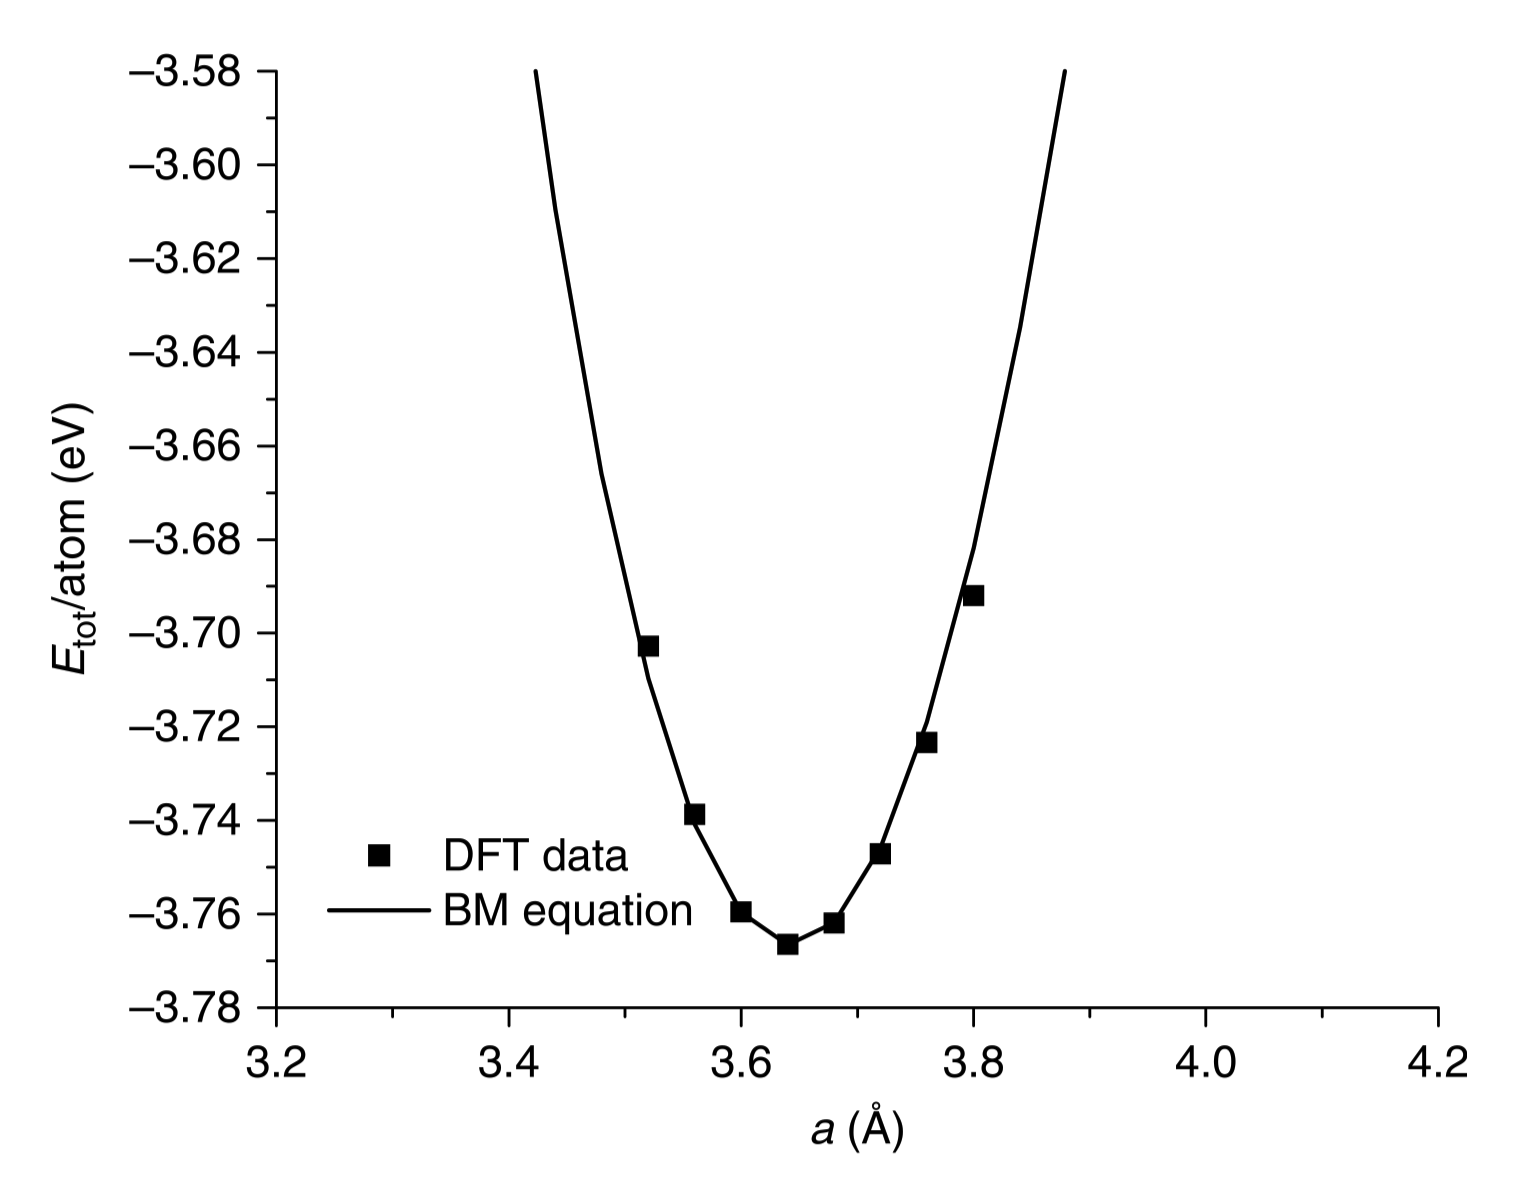
\includegraphics[width=0.45\linewidth]{lectures/figures/8_Cu_EOS.png}
            \caption{Total energy, E, of Cu in the fcc crystal structure as a function of the lattice parameter, a. Data points are from DFT calculations and the dashed curve is the Birch–Murnaghan equation of state.\cite{shollDensityFunctionalTheory2023}}
        \end{figure}
    \end{frame}


    \begin{frame}{Optimization Algorithms}

        \begin{columns}
            \column{0.6\textwidth}
            Most codes supports many options. Some common ones include:
            \begin{itemize}
                \item Quasi-newton: Newton's method for finding local minima/maxima, but with approximations for the derivatives of the functions. E.g., BFGS, FIRE, etc.
                \item Conjugate gradient: Typically requires fewer steps to reach minima.
            \end{itemize}
            \column{0.4\textwidth}
            \begin{figure}
                \centering
                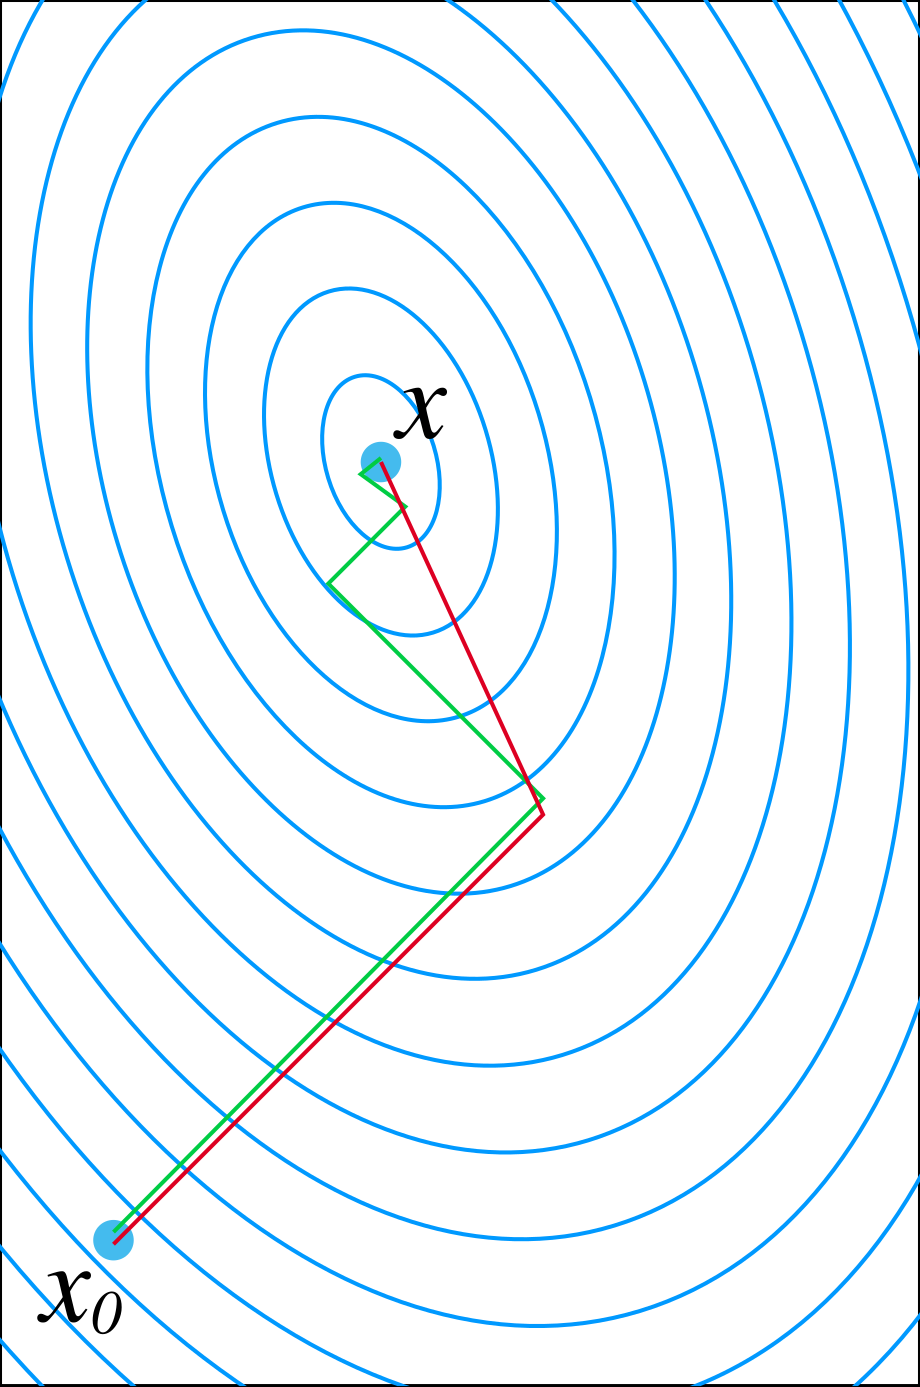
\includegraphics[width=0.5\linewidth]{lectures/figures/8_conjugate_gradient.png}
                \caption{Convergence of gradient descent (green) and conjugate gradient (red) for minimizing a quadratic function.}
            \end{figure}
        \end{columns}

    \end{frame}

    \begin{frame}{Phase transitions under pressure}

        \begin{figure}
            \centering
            \begin{subfigure}{0.45\textwidth}
                \centering
                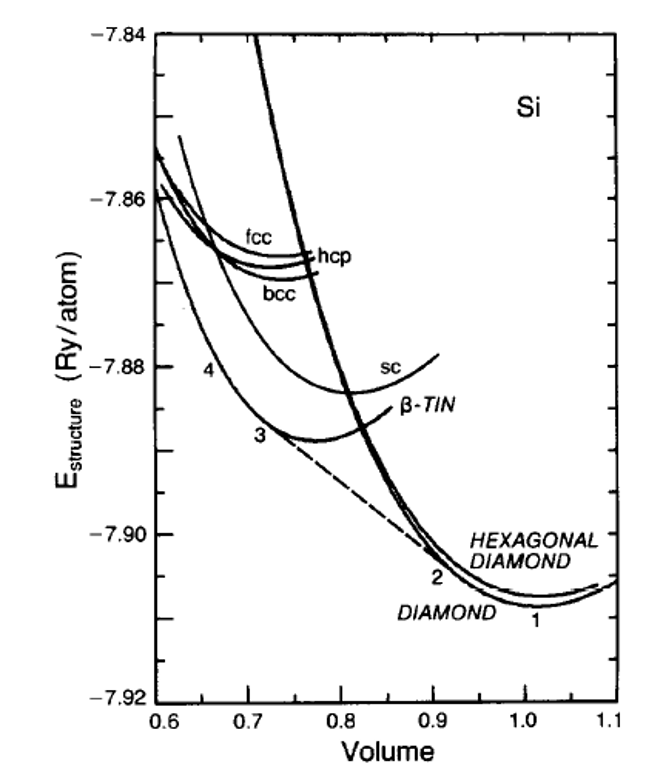
\includegraphics[width=0.7\linewidth]{lectures/figures/5_phase_diagram_si.png}
                \caption{Phase diagram of Si from LDA.\cite{yinTheoryStaticStructural1982} Transition pressure given by $P = -\frac{\partial E}{\partial V}$.}
            \end{subfigure}
            \begin{subfigure}{0.45\textwidth}
                \centering
                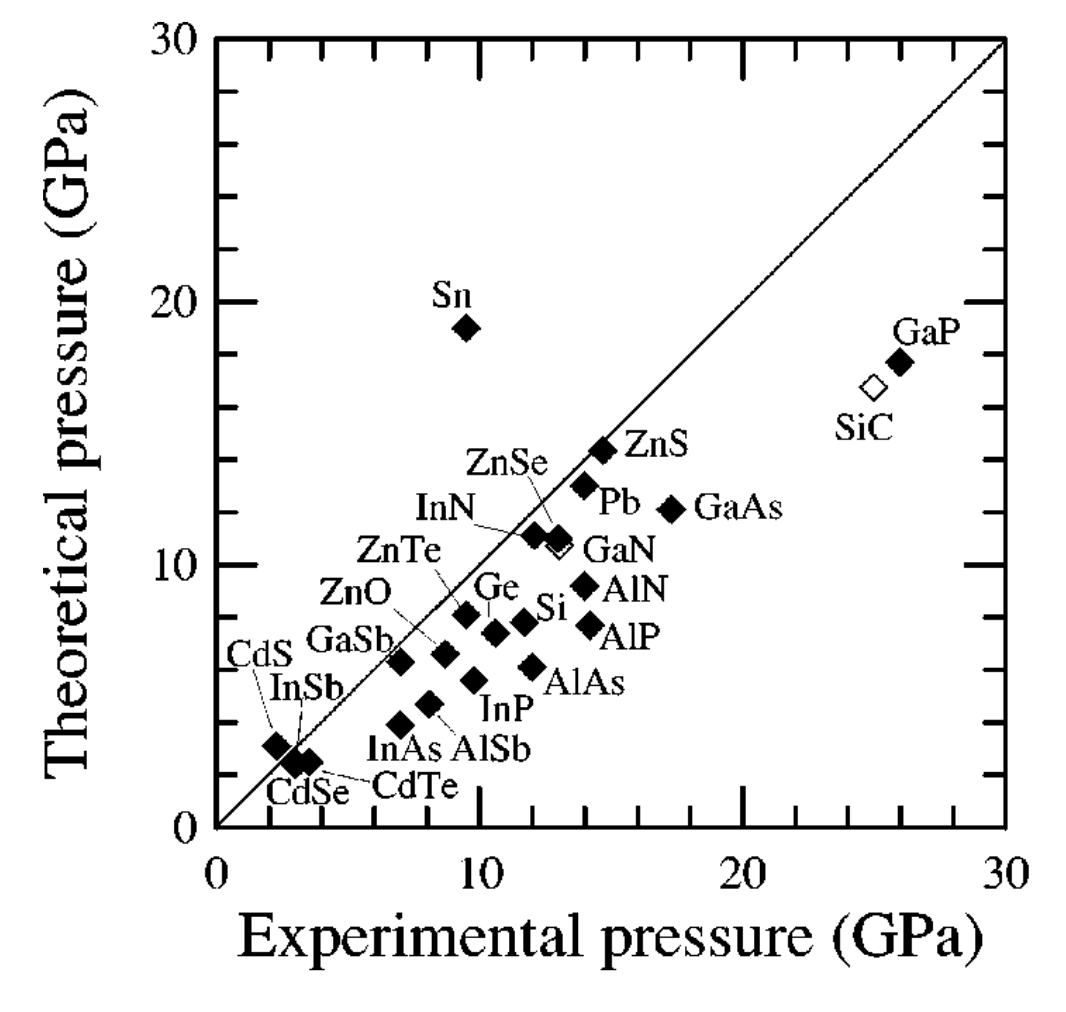
\includegraphics[width=0.8\linewidth]{lectures/figures/8_phase_transition_pressure_III_V_and_II-VI.png}
                \caption{LDA vs experimental transition pressures for the first phase transition in group-IVA elements and IIIA–VA and IIB–VIA compounds.\cite{mujicaHighpressurePhasesGroupIV2003}}
            \end{subfigure}
        \end{figure}

    \end{frame}

    \begin{frame}{Magnetism can play a huge role in geometry and phase stability}
        \begin{figure}
            \centering
            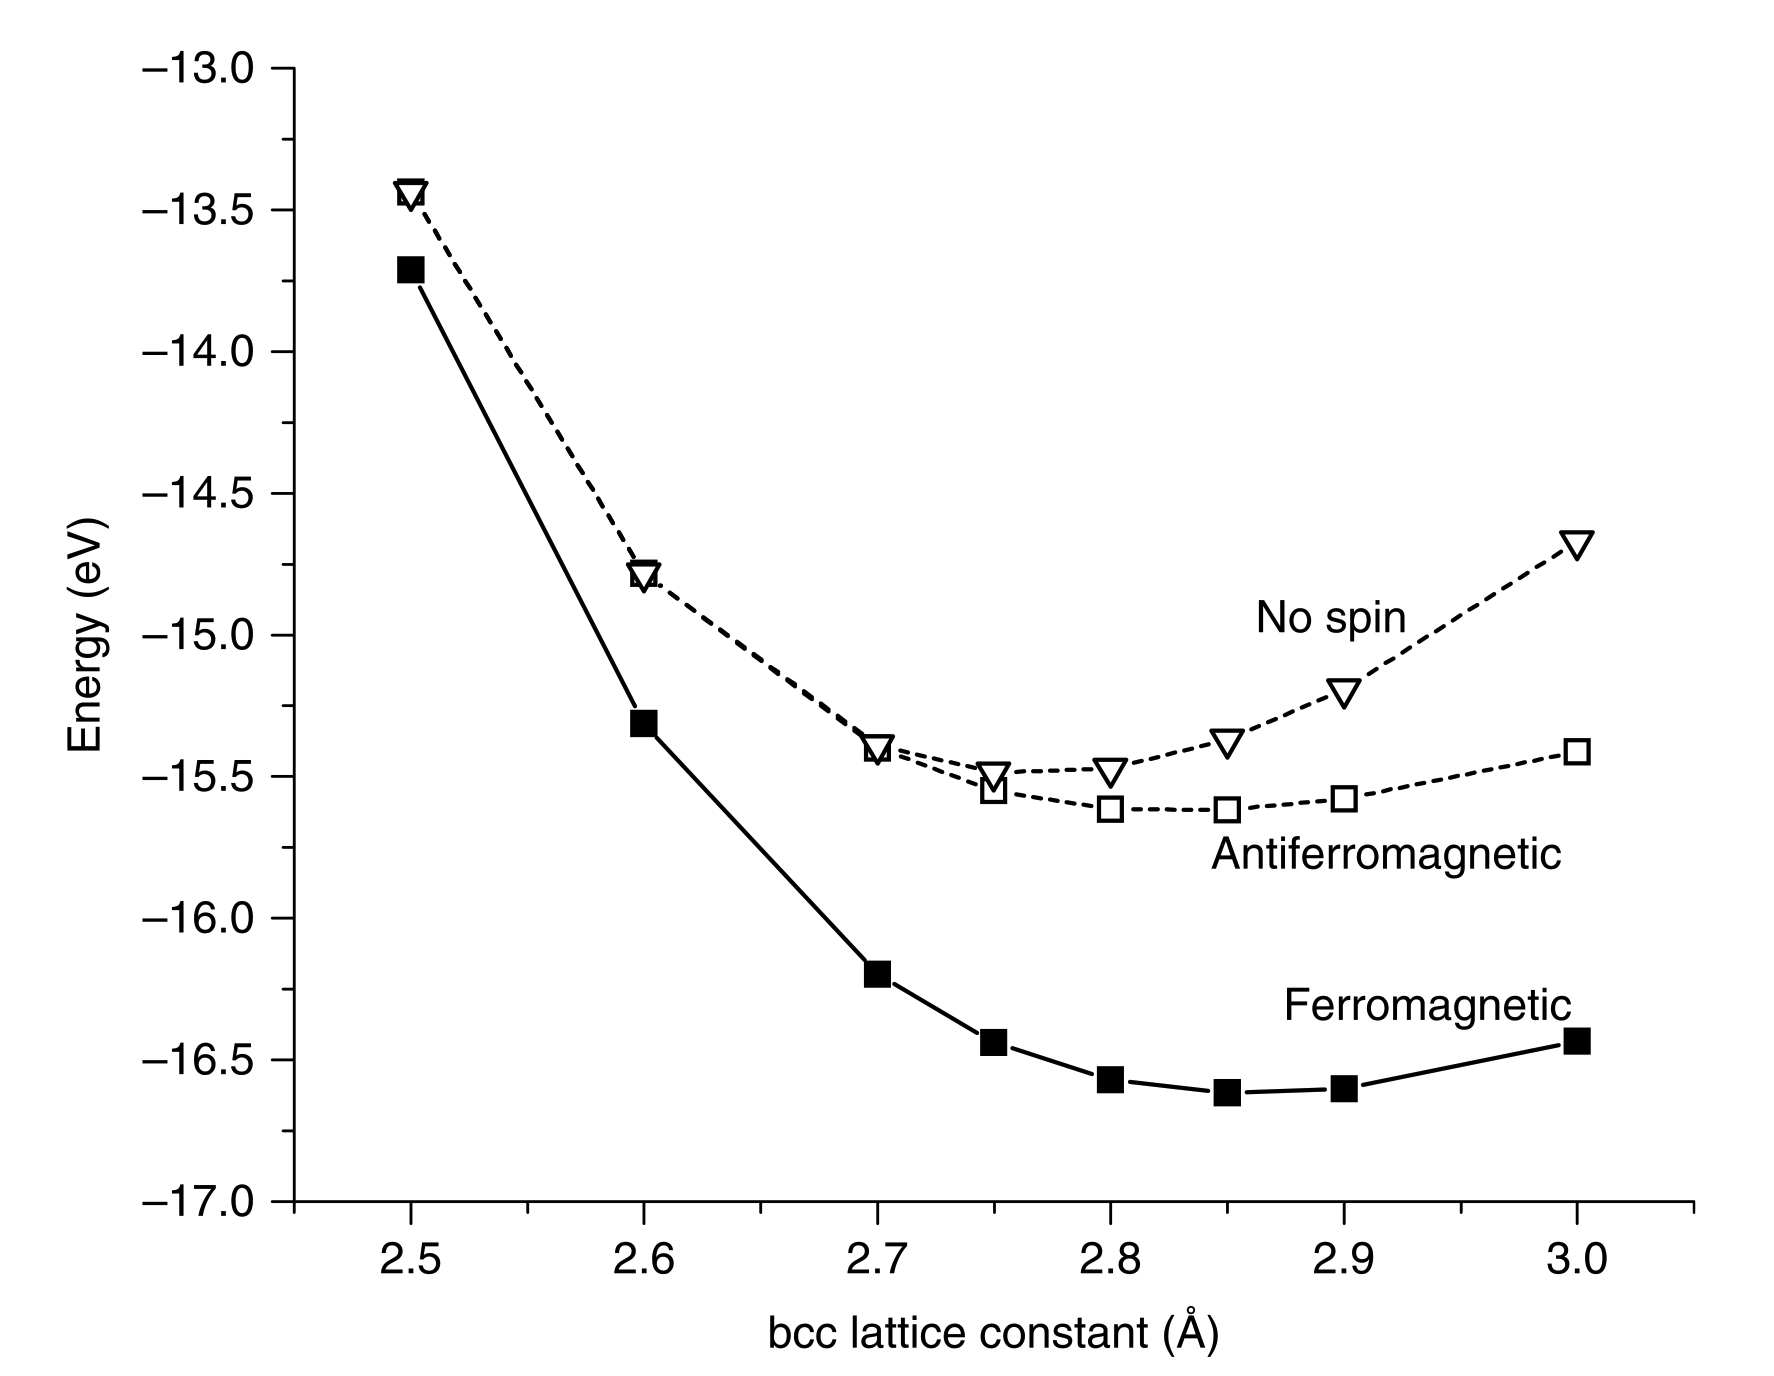
\includegraphics[width=0.5\linewidth]{lectures/figures/8_magnetism_Fe.png}
            \caption{DFT energy of bcc Fe as a function of the Fe lattice constant with several different spin states. Reproduced from \cite{shollDensityFunctionalTheory2023}.}
        \end{figure}
    \end{frame}

    \begin{frame}{Mechanical Properties}
        \begin{columns}
            \column{0.5\textwidth}
            \begin{equation*}
                K = -V\frac{\partial P}{\partial V} = V \frac{\partial^2 E}{\partial V^2}, c_{ijkl} = \frac{\partial^2 E}{\partial \varepsilon_{ij}\partial \varepsilon_{kl}}
            \end{equation*}
            \begin{figure}
                \centering
                \begin{subfigure}{0.45\textwidth}
                    \centering
                    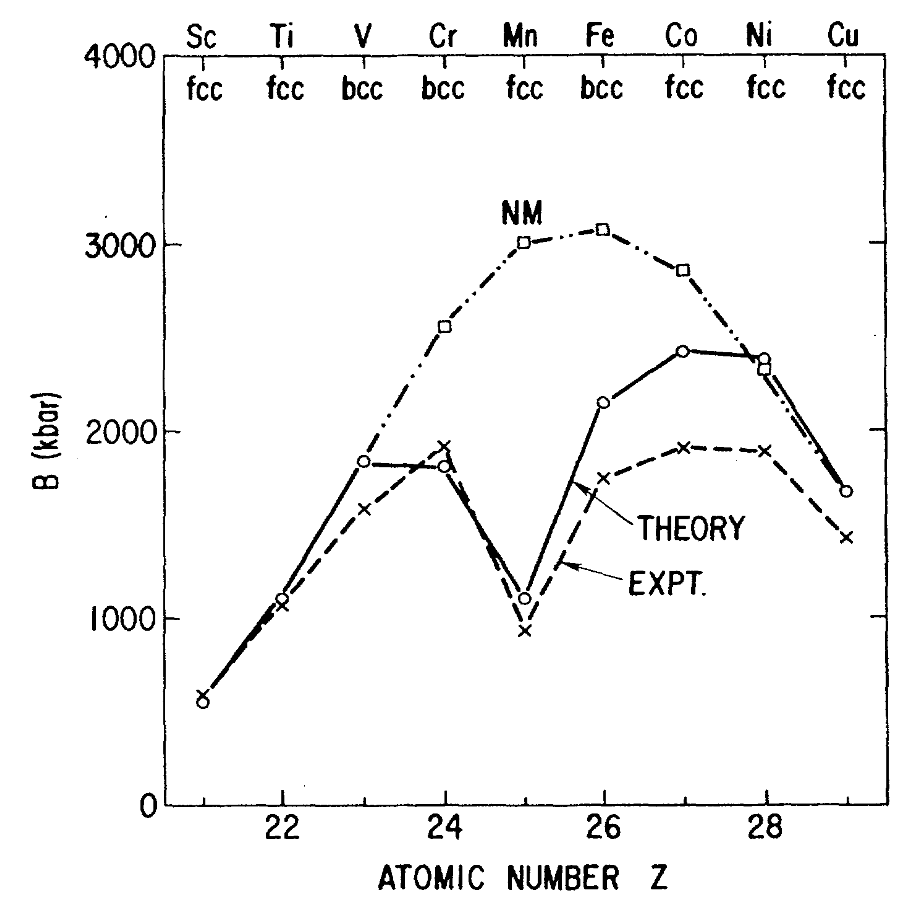
\includegraphics[width=\linewidth]{lectures/figures/8_3D_TM_Bulk_Moduli.png}
                    \caption{3d}
                \end{subfigure}
                \begin{subfigure}{0.45\textwidth}
                    \centering
                    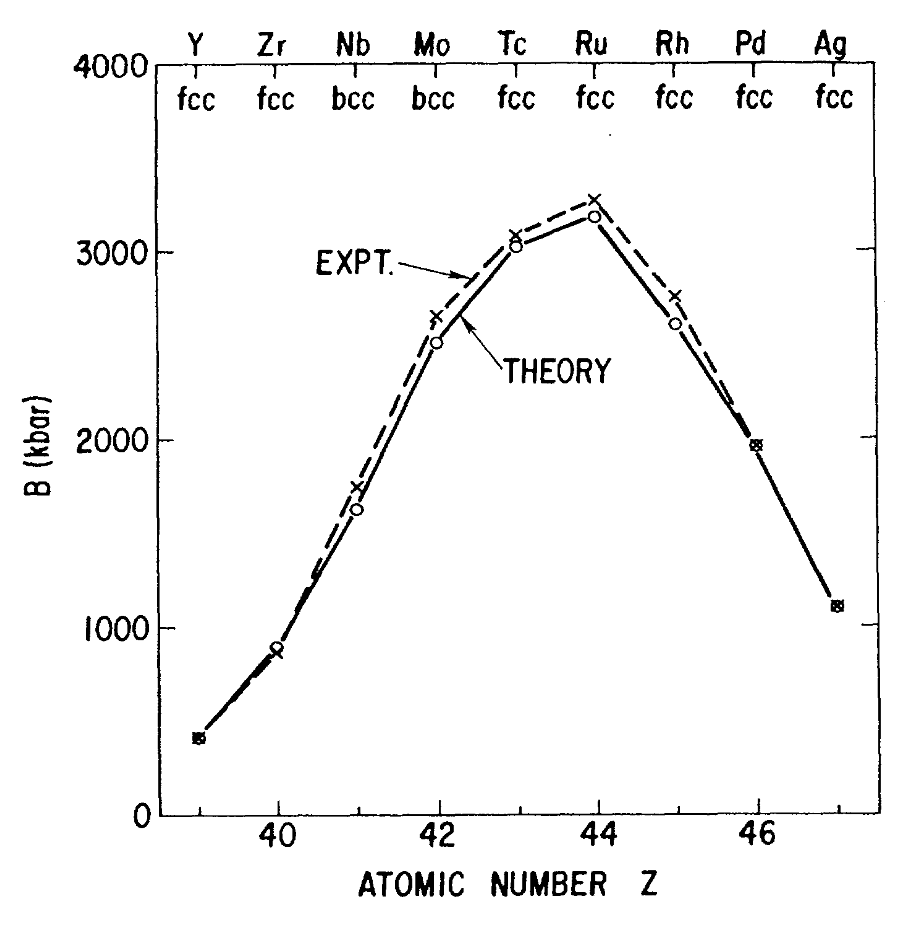
\includegraphics[width=\linewidth]{lectures/figures/8_4D_TM_Bulk_Moduli.png}
                    \caption{4d}
                \end{subfigure}
                \caption{Bulk moduli of 3d and 4d metals.\cite{moruzziTrendsBulkModuli1993}}
            \end{figure}

            \column{0.5\textwidth}

            \begin{figure}
                \centering
                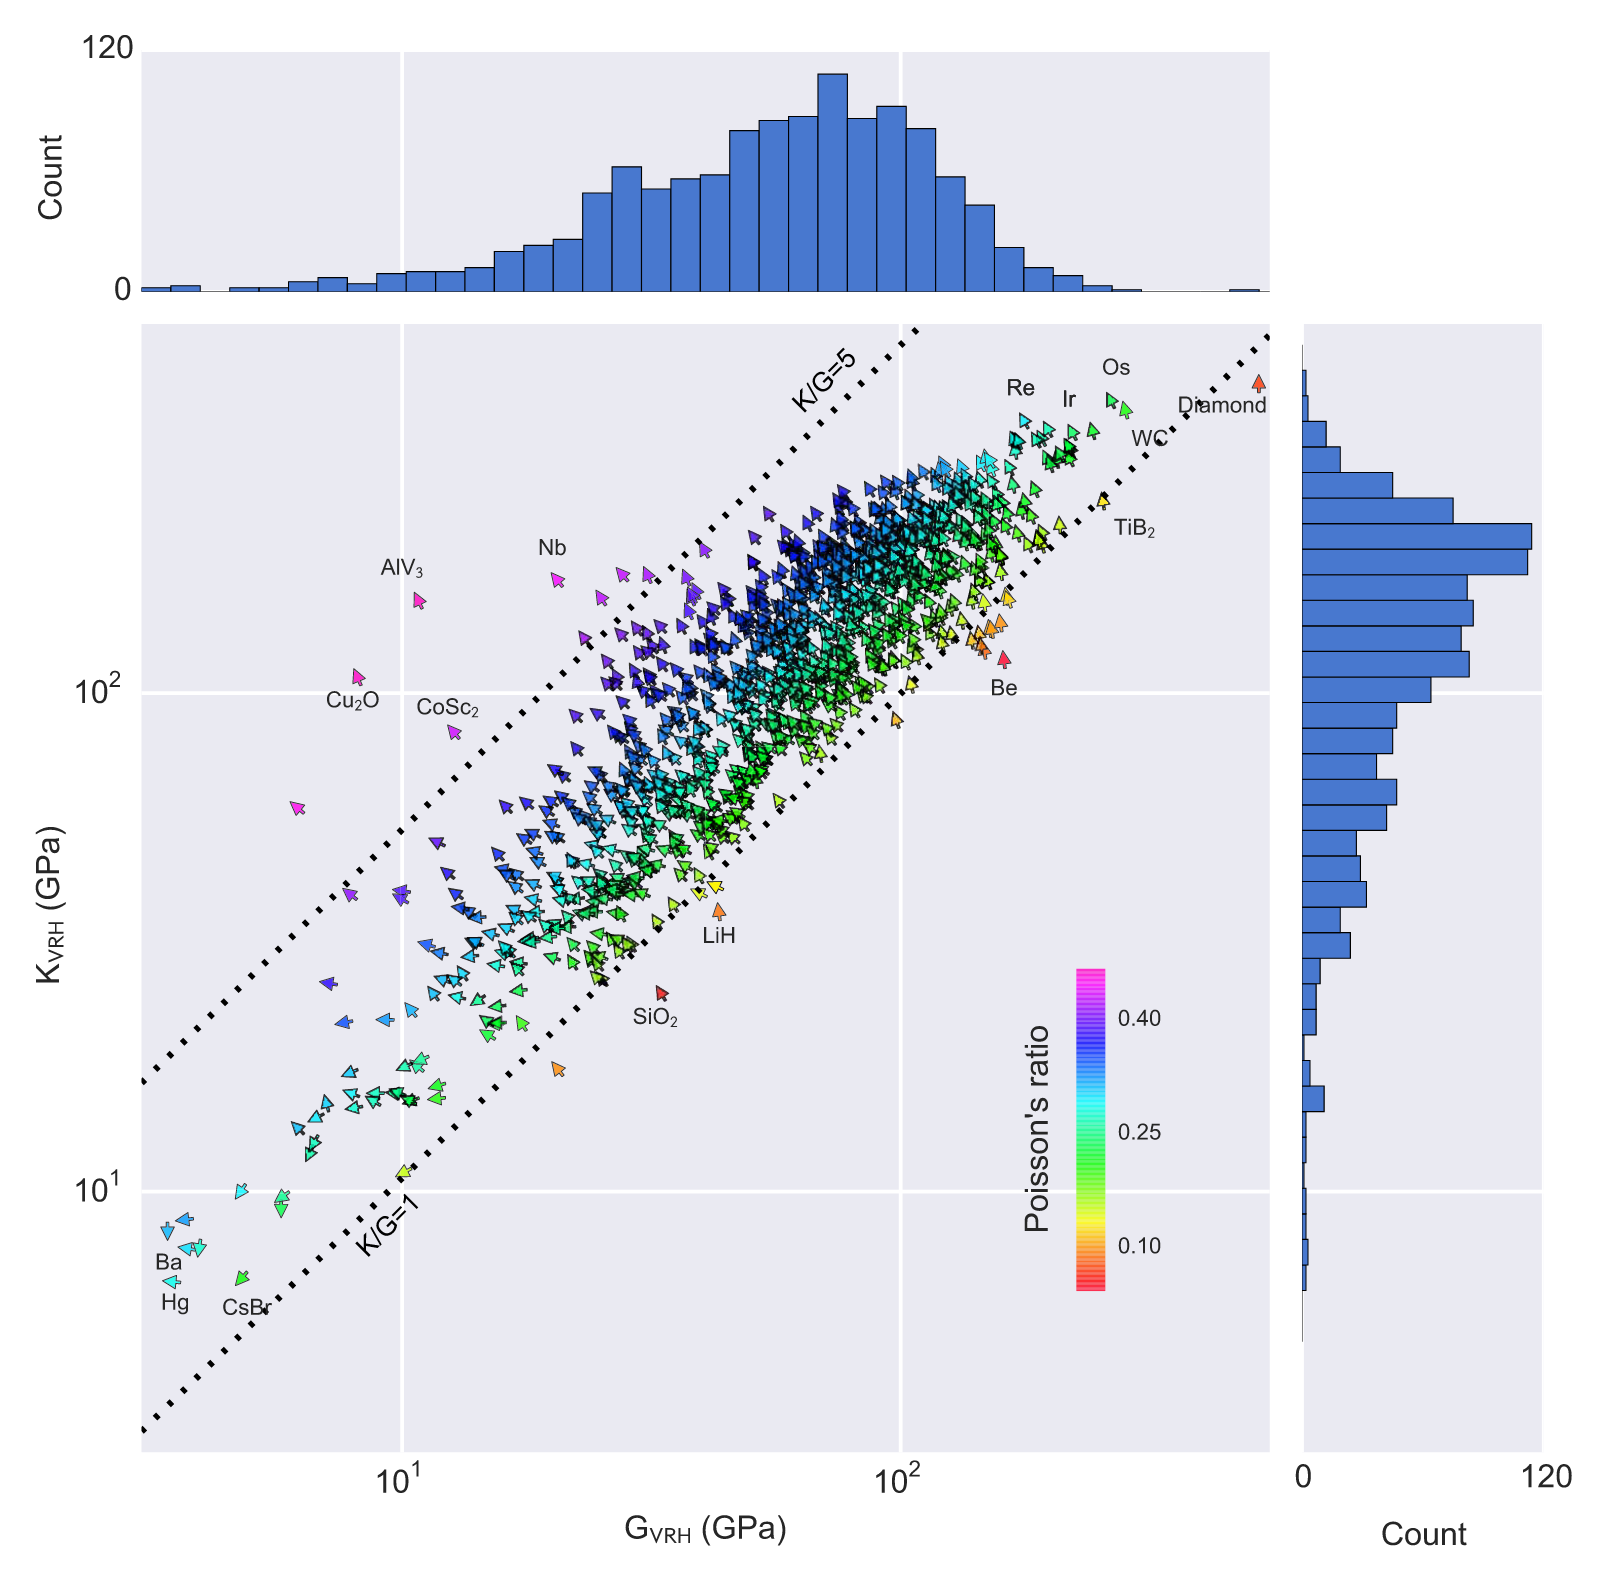
\includegraphics[width=0.7\linewidth]{lectures/figures/8_MP_Elastic_Moduli.png}
                \caption{Distribution of DFT volume per atom, Poisson ratio, bulk modulus and shear modulus.\cite{dejongChartingCompleteElastic2015}}
            \end{figure}

        \end{columns}
    \end{frame}

    \begin{frame}{Electronic Structure}
        \begin{equation*}
            \rho(E) = \frac{\Omega}{(2\pi)^d} \int_{BZ} \delta(\varepsilon_{i, \vec{k}}-E) dE
        \end{equation*}

        \begin{figure}
            \centering
            \begin{subfigure}{0.3\textwidth}
                \centering
                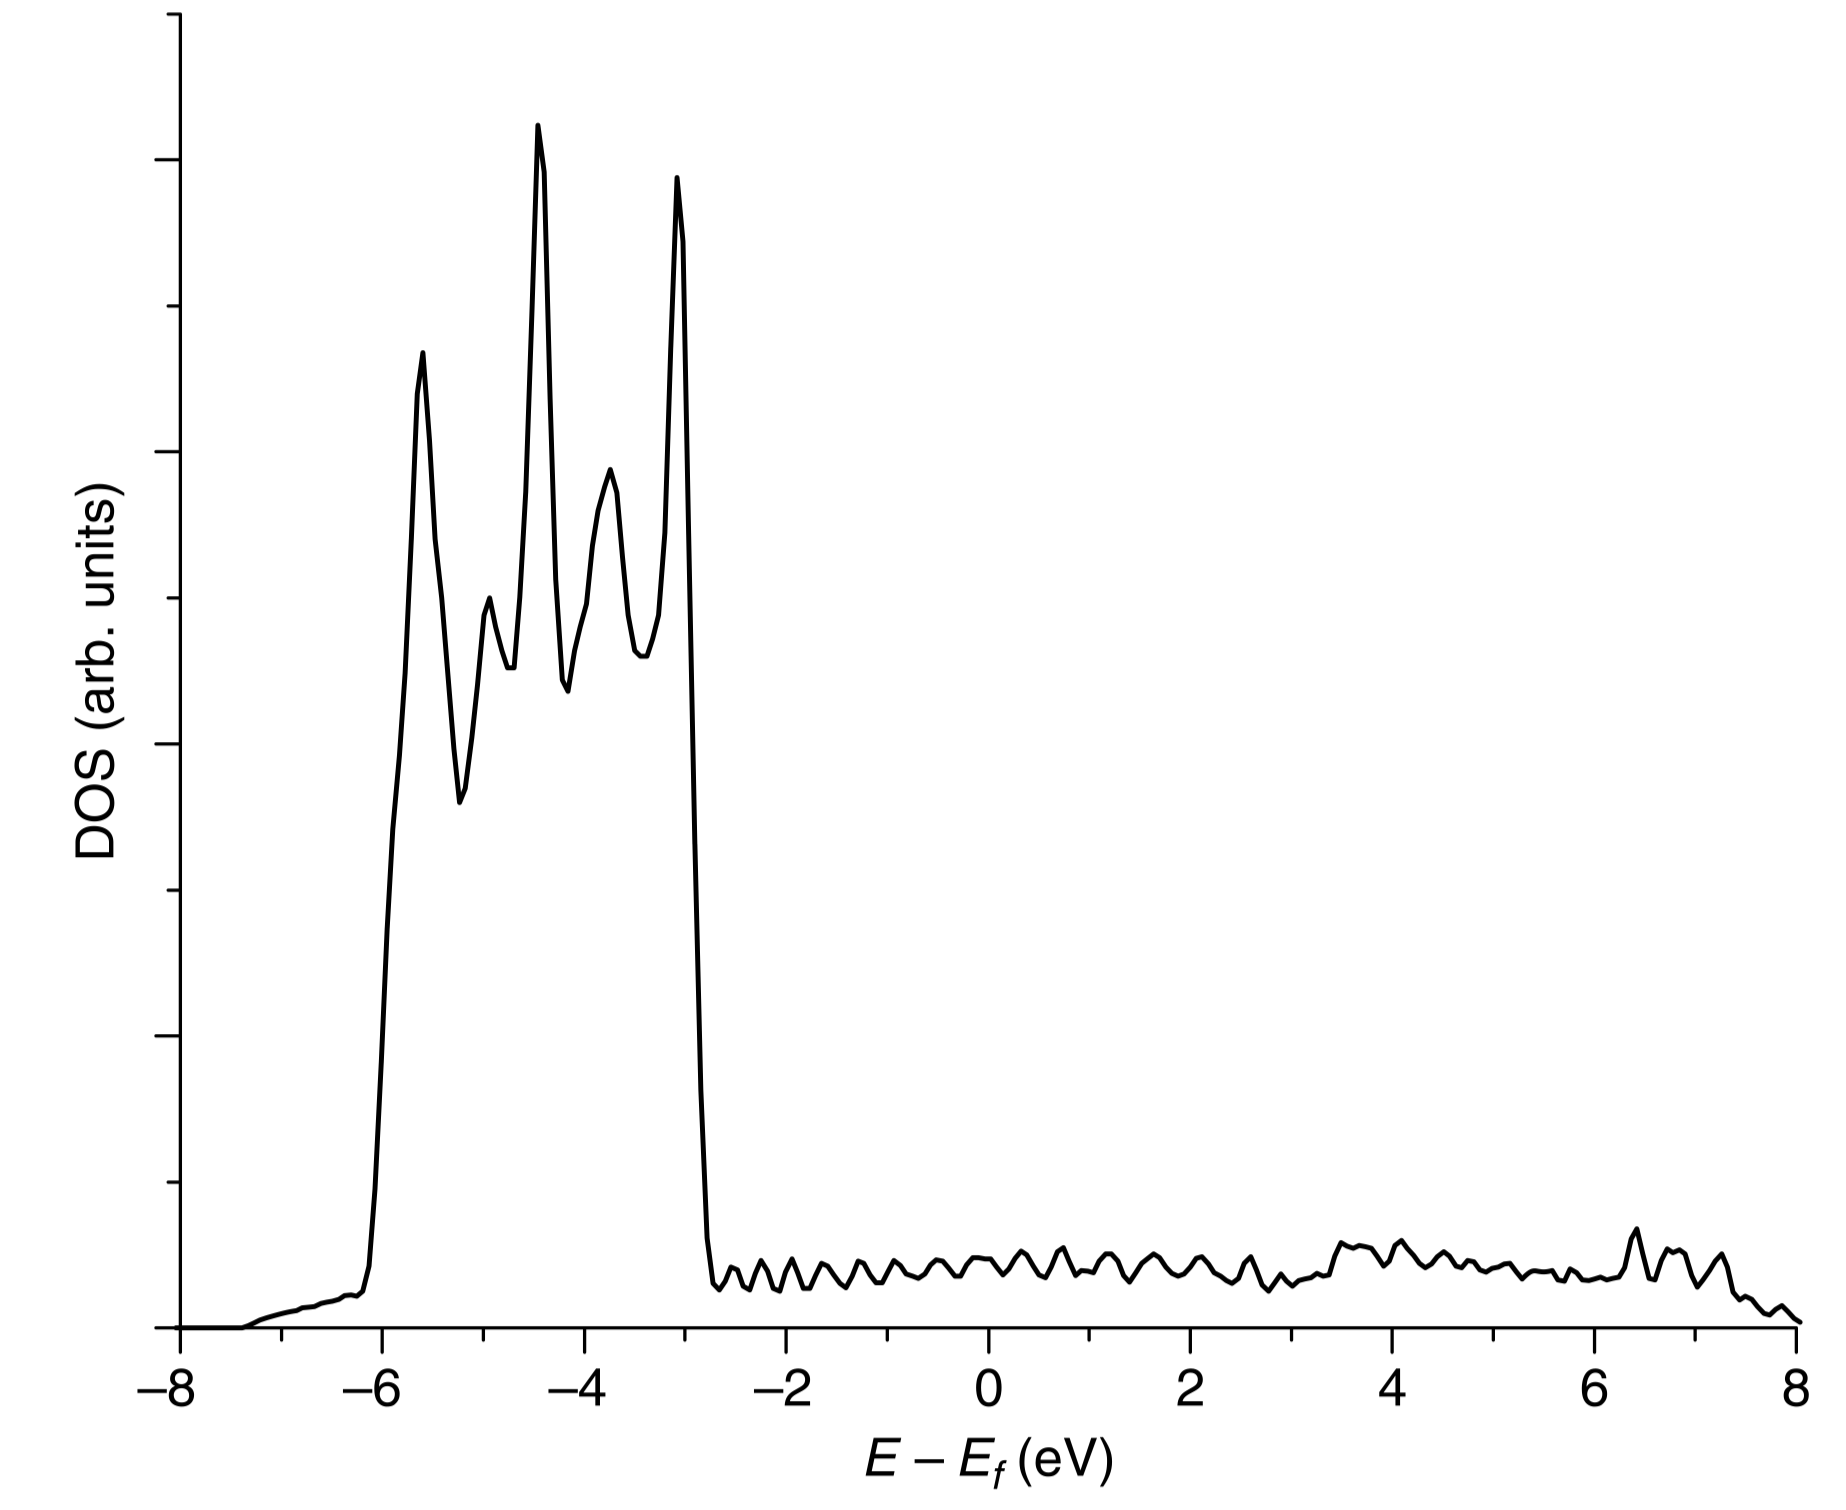
\includegraphics[width=\linewidth]{lectures/figures/8_DOS_Ag.png}
                \caption{Ag, $24 \times 24 \times 24$ k points.}
            \end{subfigure}
            \begin{subfigure}{0.3\textwidth}
                \centering
                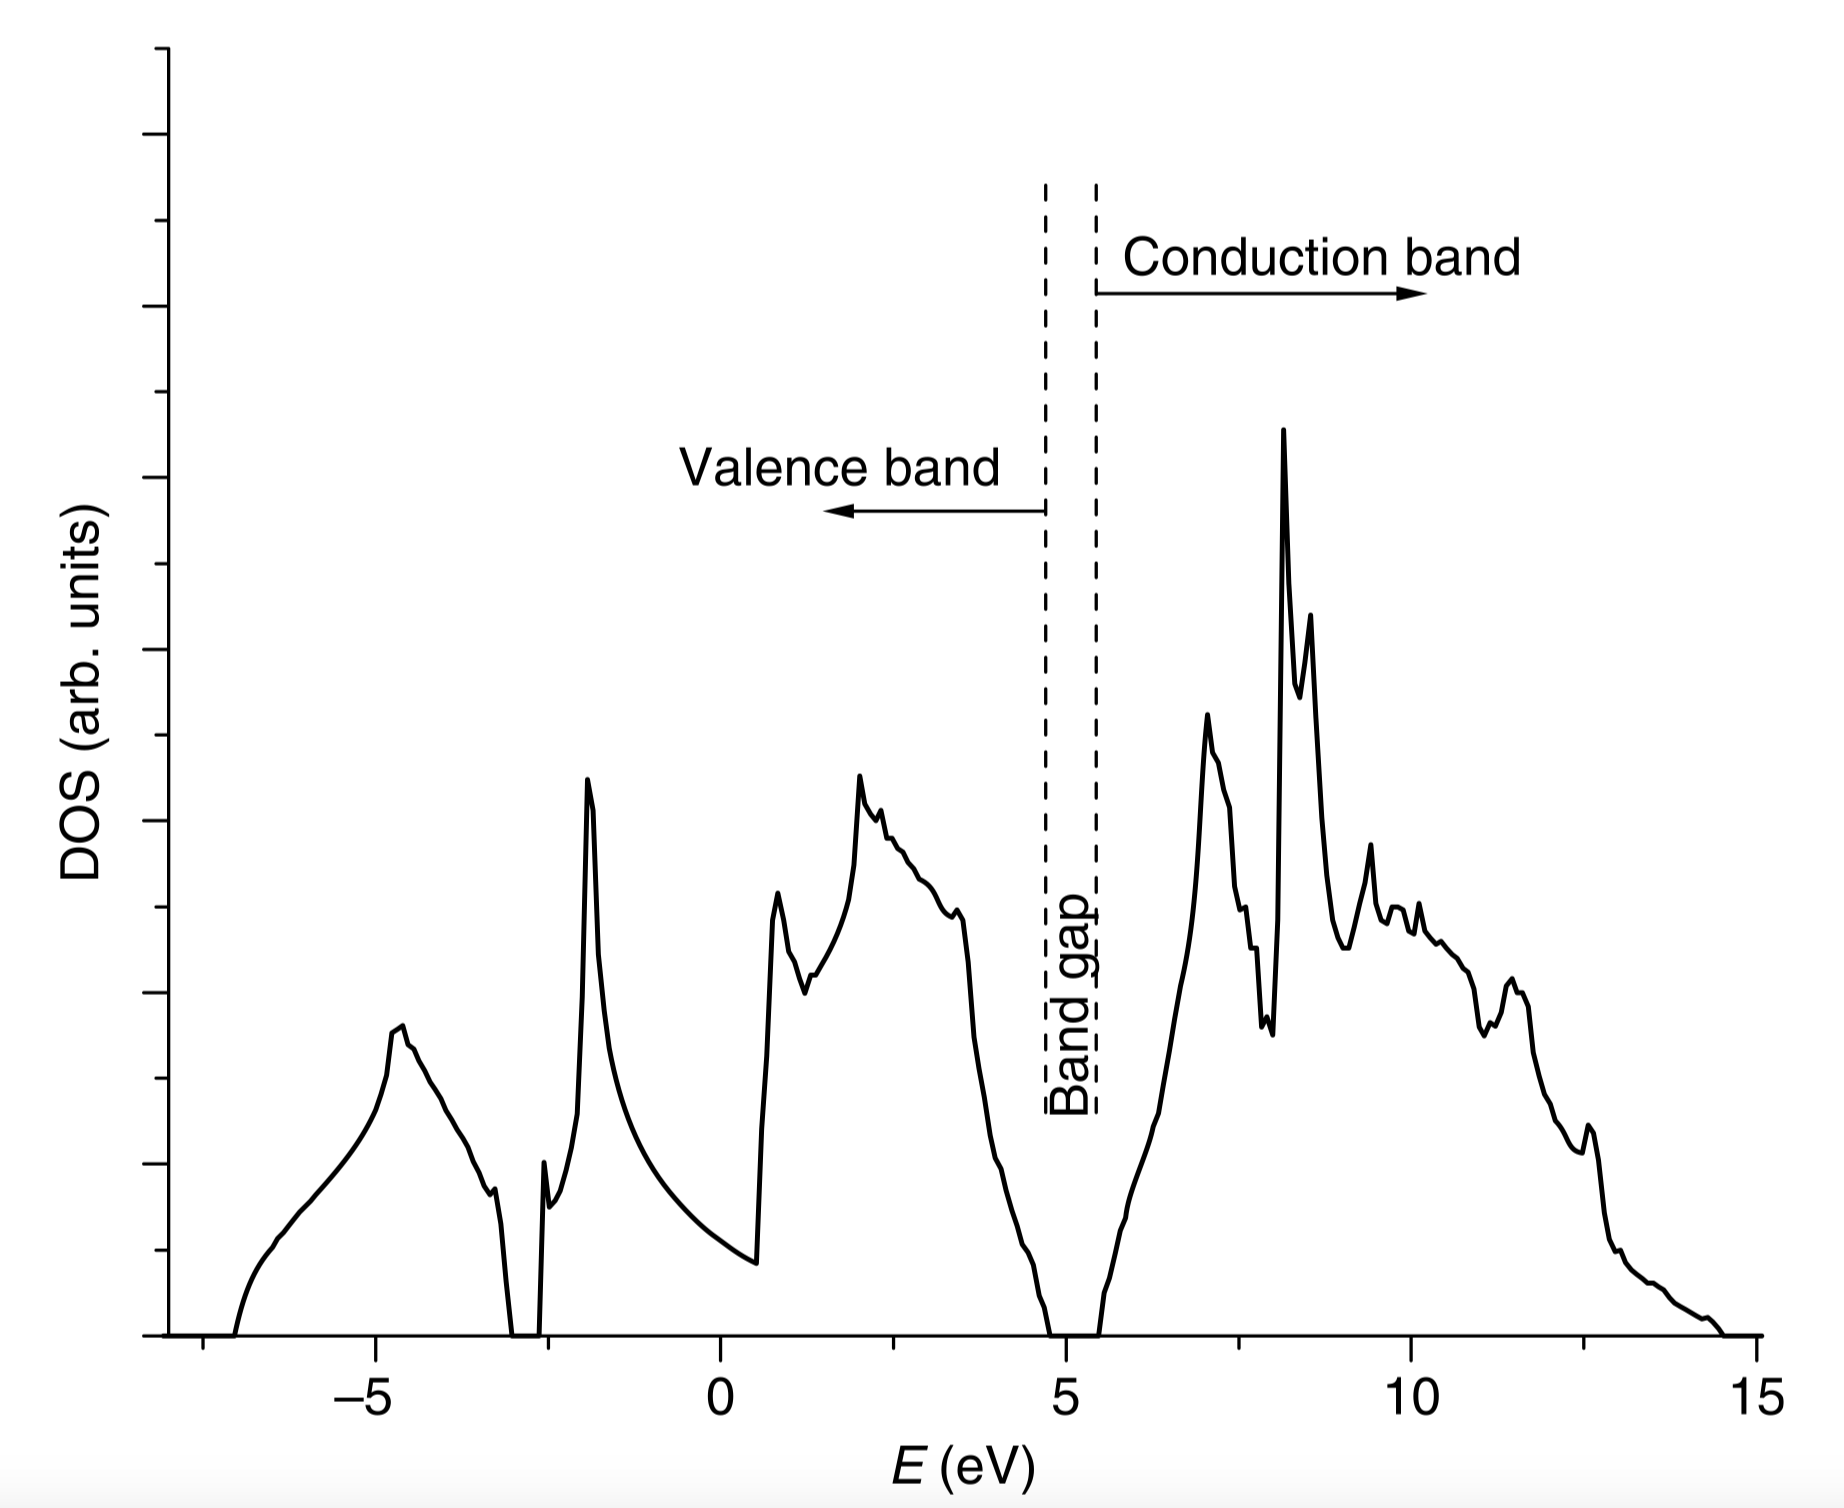
\includegraphics[width=\linewidth]{lectures/figures/8_DOS_Si.png}
                \caption{Si}
            \end{subfigure}
            \caption{Electronic density of states (DOS) from PBE calculations.\cite{shollDensityFunctionalTheory2009} Note that the significant underestimation of the band gap of Si.}
            \label{fig}
        \end{figure}
    \end{frame}

    \begin{frame}{Bandstructure}
        \begin{figure}
            \centering
            \begin{subfigure}{0.45\textwidth}
                \centering
                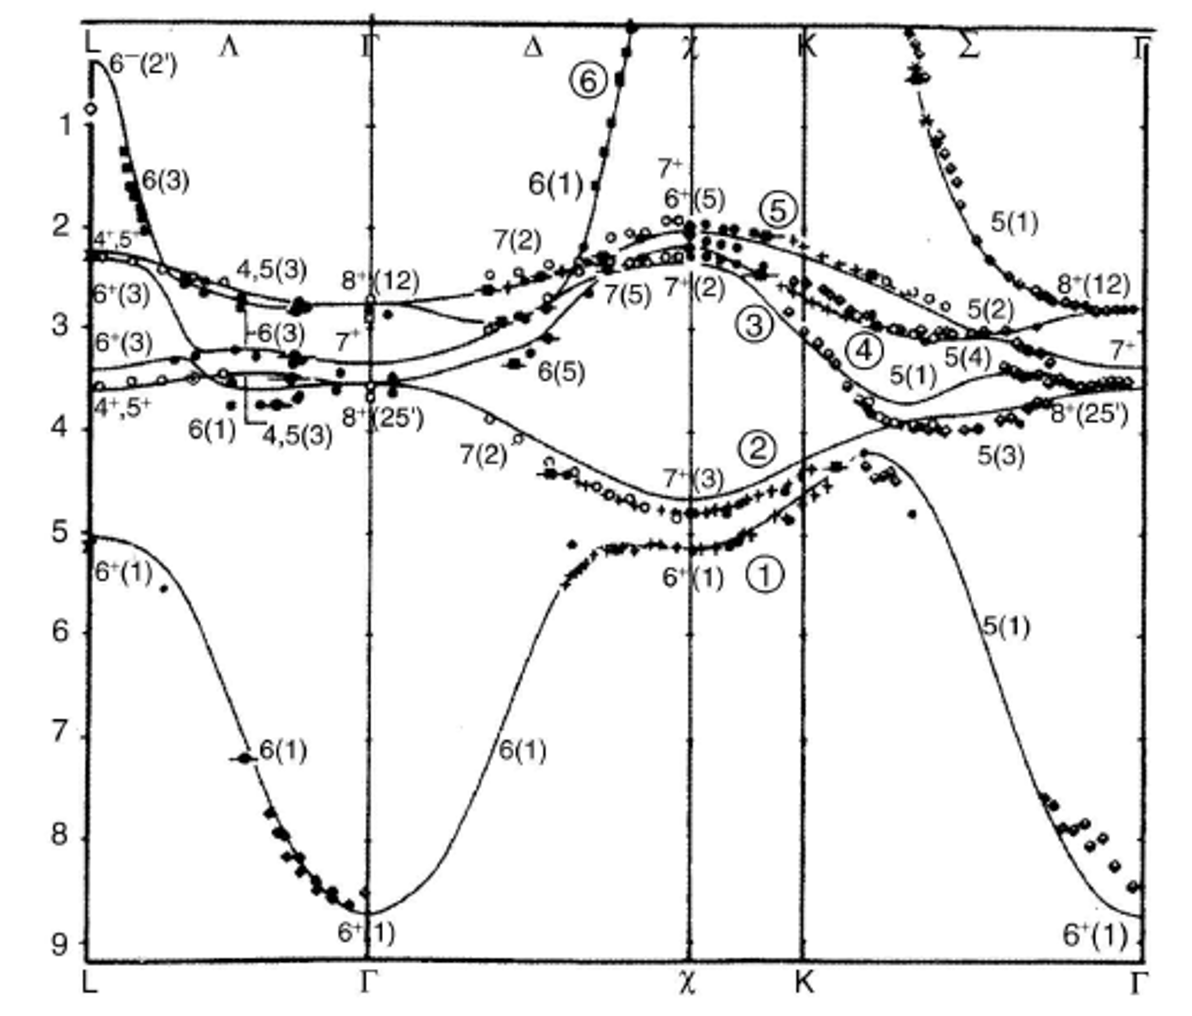
\includegraphics[width=0.8\linewidth]{lectures/figures/8_Bandstructure_Cu.png}
                \caption{Experimental energy bands of Cu measured by angle-resolved photoemission compared with the classic APW calculations.\cite{martinElectronicStructureBasic2004}}
            \end{subfigure}
            \begin{subfigure}{0.5\textwidth}
                \centering
                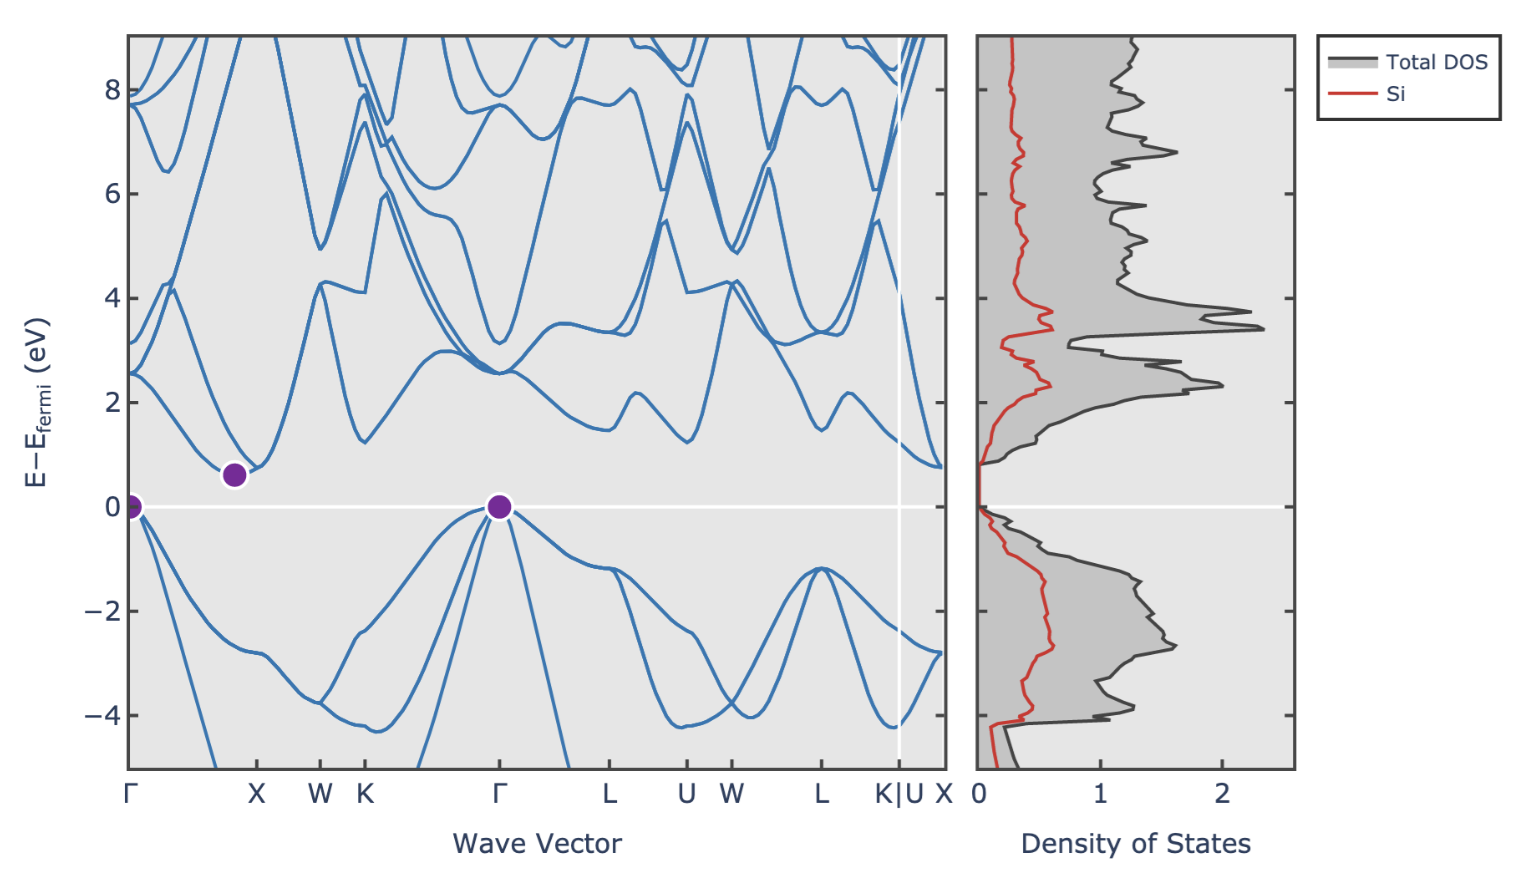
\includegraphics[width=\linewidth]{lectures/figures/8_Bandstructure_Si.png}
                \caption{Si.\cite{jainCommentaryMaterialsProject2013}}
            \end{subfigure}
            \caption{Band structure from PBE calculations.}
            \label{fig}
        \end{figure}
    \end{frame}

    \begin{frame}{High-throughput Bandstructure Computations}
        \begin{figure}
            \centering
            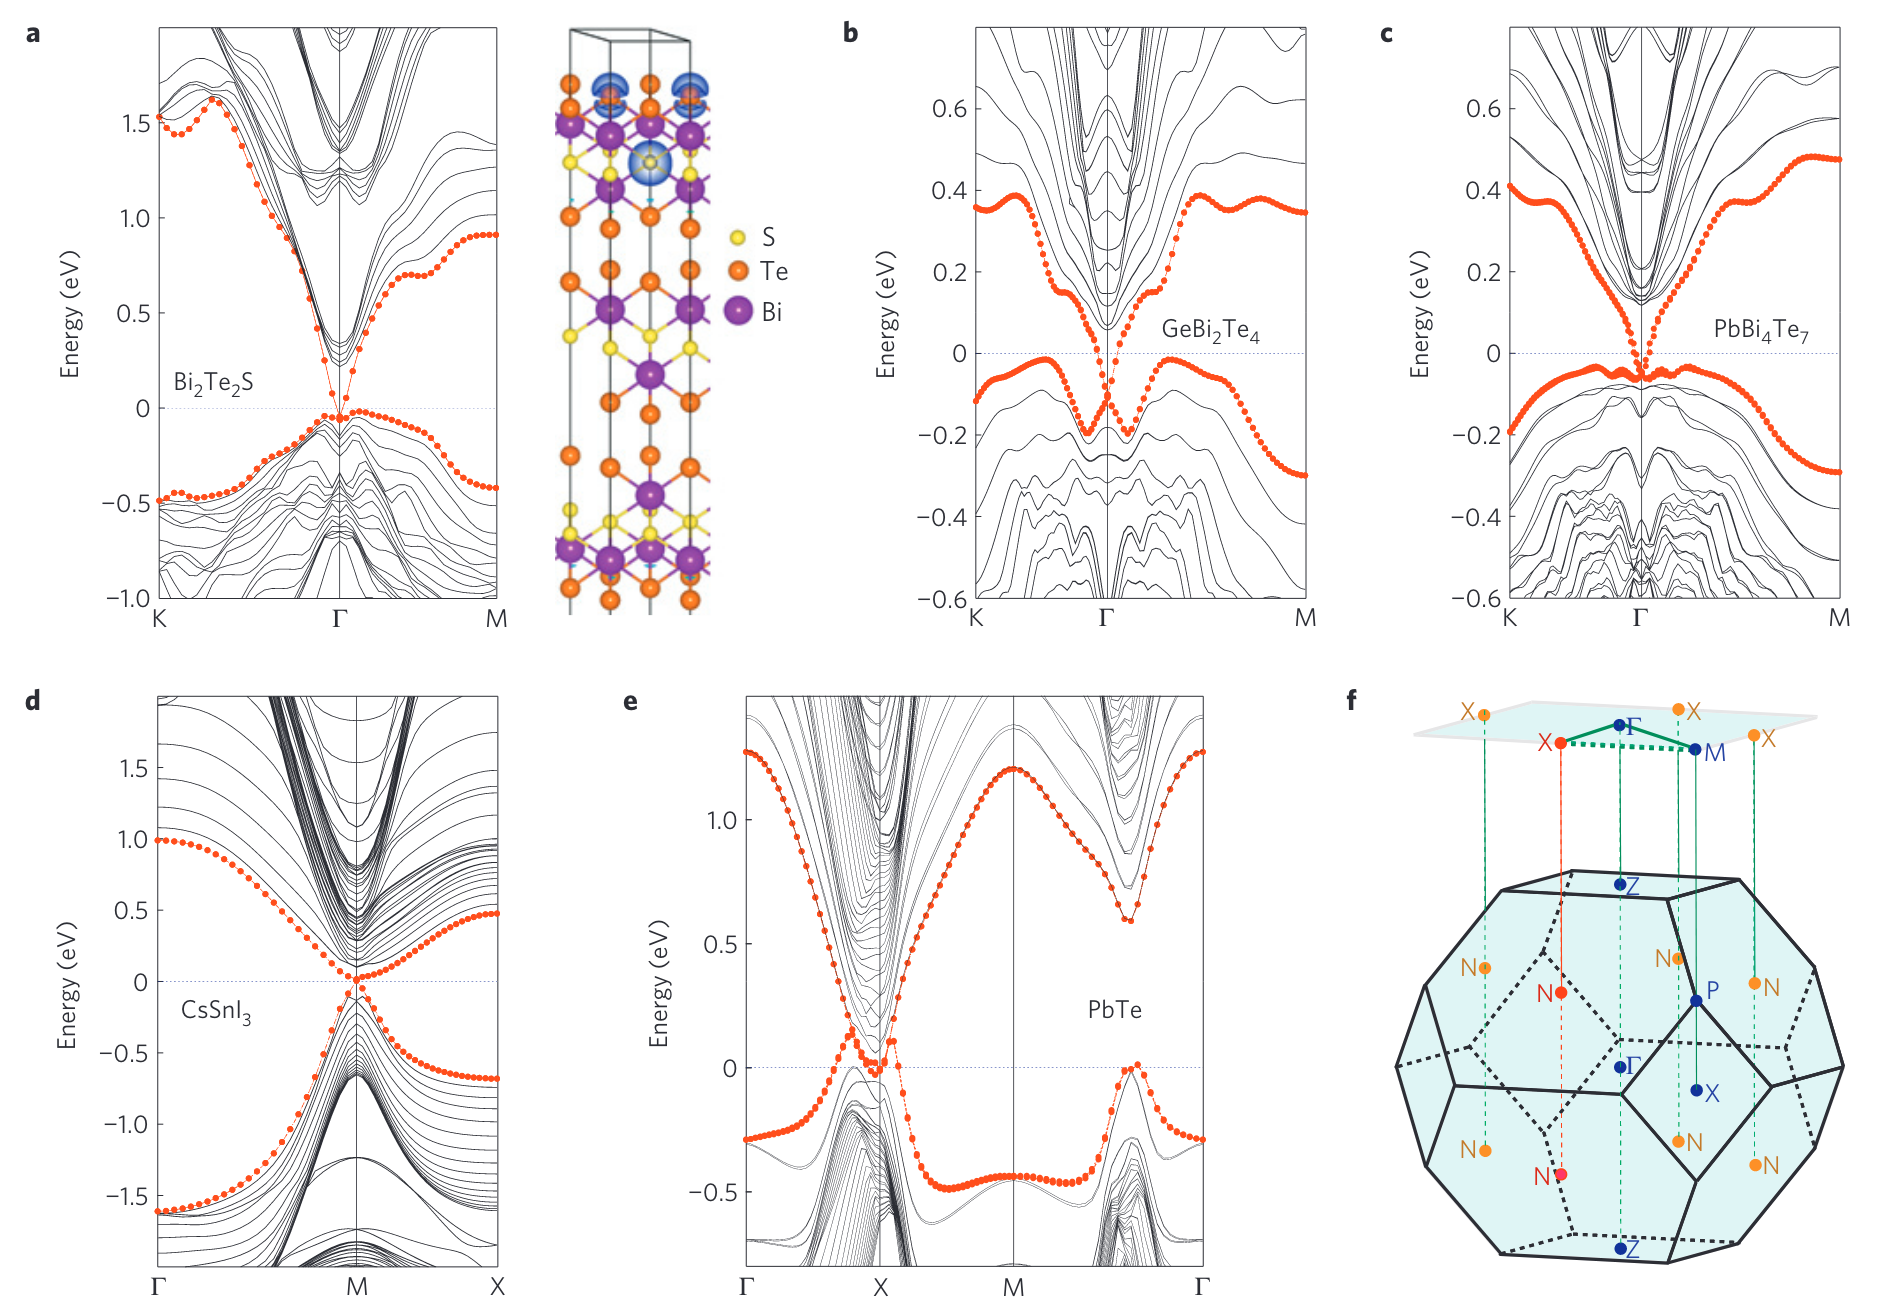
\includegraphics[width=0.5\linewidth]{lectures/figures/8_HT_Bandstructure.png}
            \caption{High-throughput 2D surface electronic structure for topological insulators.\cite{yangSearchModelTopological2012}}
        \end{figure}
    \end{frame}

    \begin{frame}{Imperfect materials}

        Real world materials are not perfect infinite solids:
        \begin{itemize}
            \item Defects - vacancies, interstitials, substitutions, etc.
            \item Surfaces
            \item Grain boundaries
            \item Interfaces
            \item Dislocations
            \item ...
        \end{itemize}

    \end{frame}

    \begin{frame}{Modelling imperfections - The Supercell method}

        \begin{figure}
            \centering
            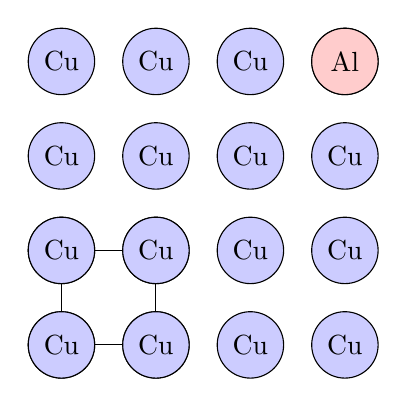
\begin{tikzpicture}[
                atom/.style={circle,draw=black,fill=white!80!blue,minimum size=24},
                dopant/.style={circle,draw=black,fill=white!80!red,minimum size=24}
            ]
                \foreach \i in {1,...,2}
                    {
                    \foreach \j in {1,...,2}
                        {
                        \pgfmathtruncatemacro{\label}{\i\j};
                        \node[atom] (\label) at (1.2*\i,1.2*\j) {Cu};

                    }
                }
% These draw commands are working as intended.
                \draw (11) -- (12);
                \draw (12) -- (22);
                \draw (21) -- (22);
                \draw (11) -- (21);
                \pause
                \foreach \i in {1,...,4}
                    {
                    \foreach \j in {1,...,4}
                        {
                        \pgfmathtruncatemacro{\label}{\i\j};
                        \node[atom] (\label) at (1.2*\i,1.2*\j) {Cu};
                    }
                }
                \pause
                \node[dopant] () at (1.2*4,1.2*4) {Al};
            \end{tikzpicture}
        \end{figure}

    \end{frame}


    \begin{frame}{Defects}
        \begin{figure}
            \centering
            \begin{subfigure}{0.3\textwidth}
                \centering
                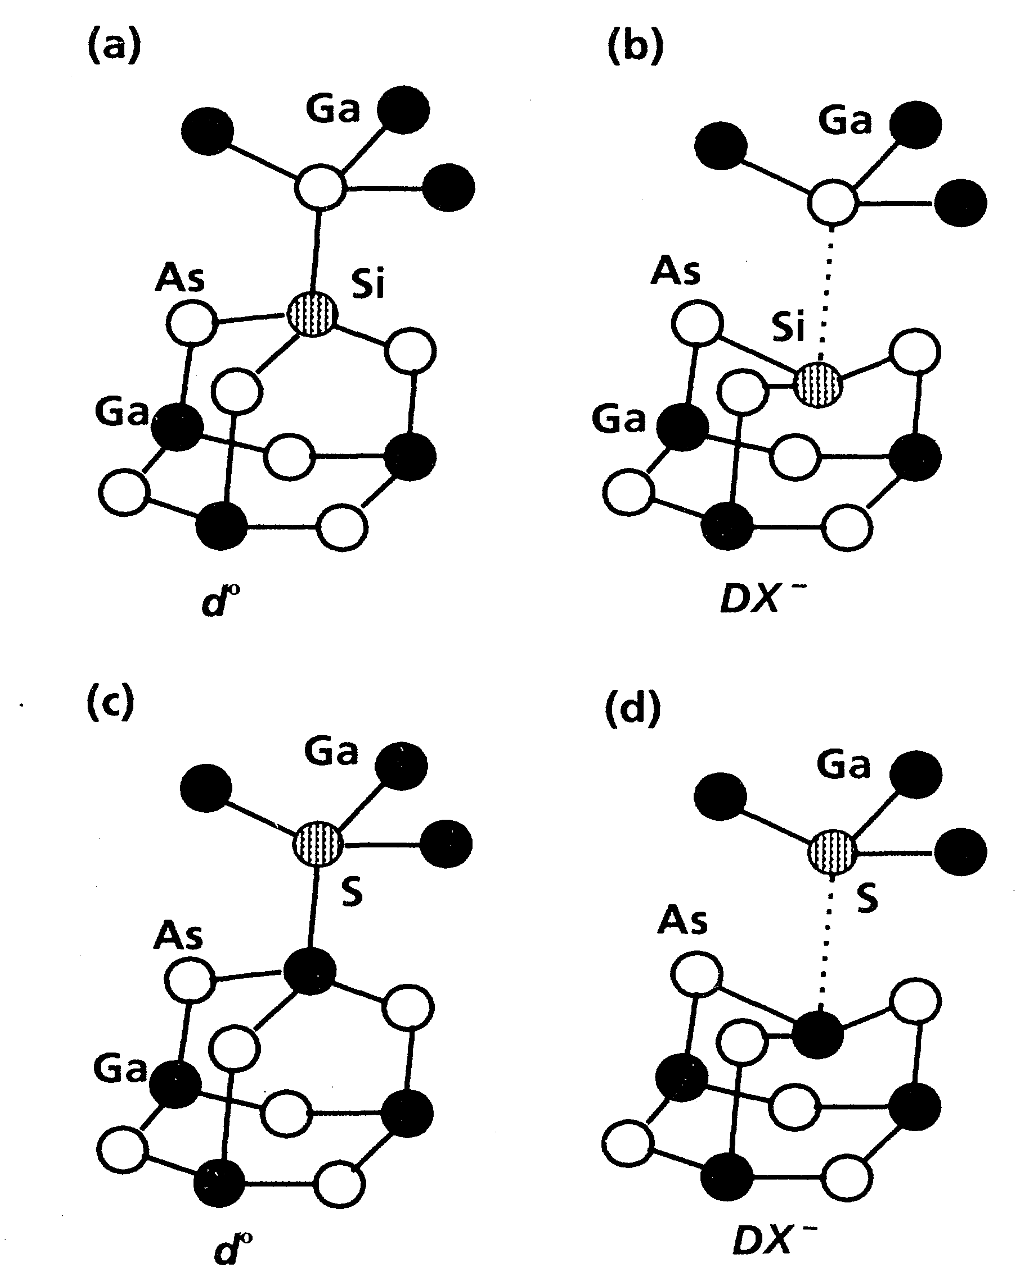
\includegraphics[width=0.7\linewidth]{lectures/figures/8_DX_Centers.png}
                \caption{Substitutional sites and the broken-bond configurations giving rise to the DX centers in Si- and S-doped \ce{Al_xGa_{1-x}As} alloys.}
            \end{subfigure}
            \begin{subfigure}{0.65\textwidth}
                \centering
                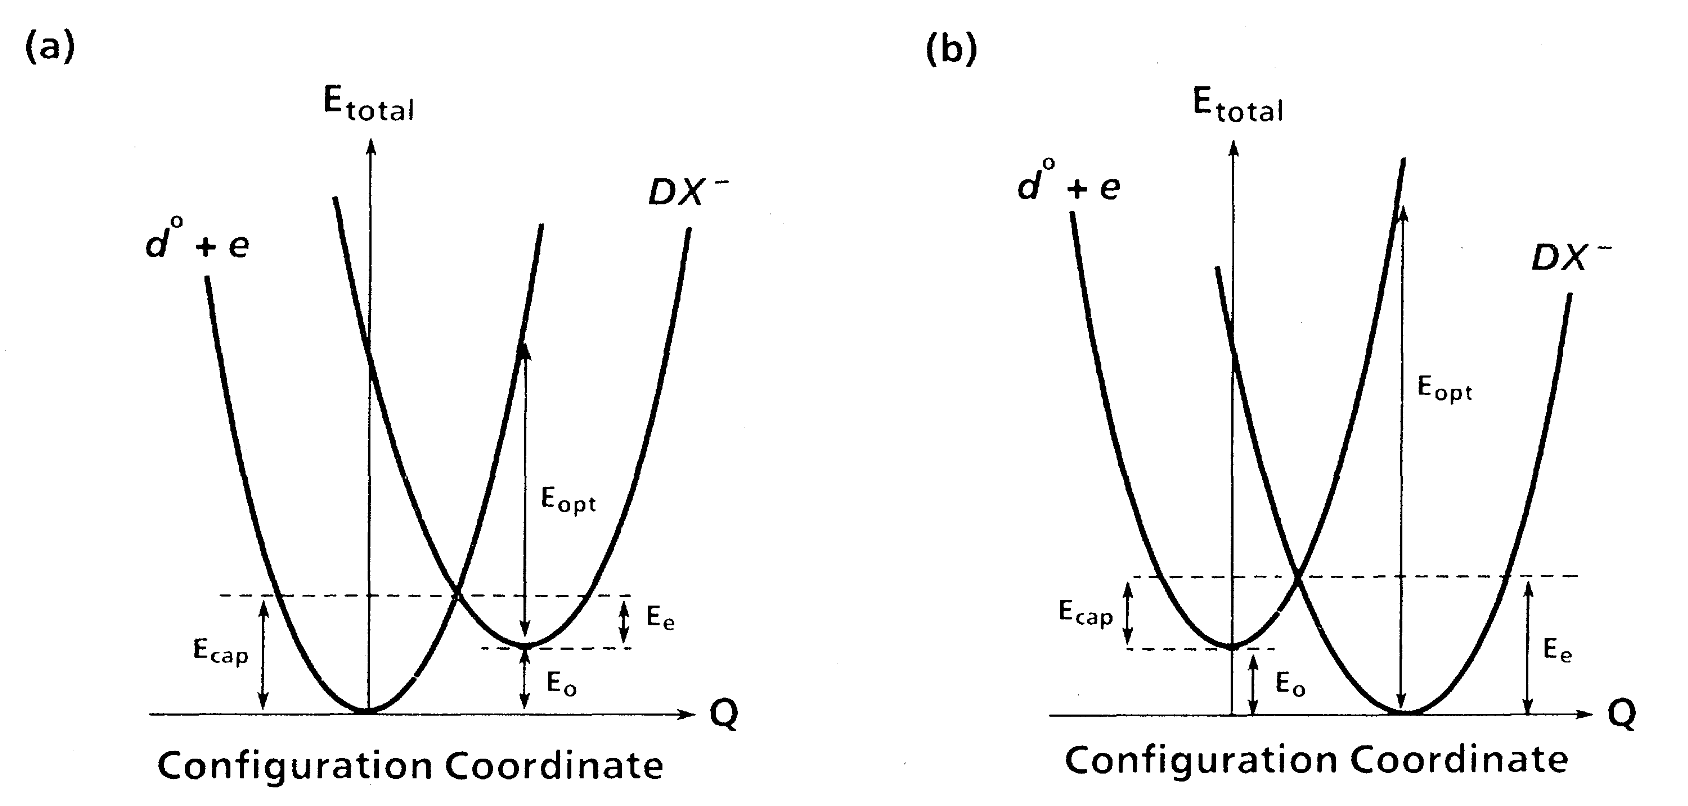
\includegraphics[width=\linewidth]{lectures/figures/8_Configuration_Diagram.png}
                \caption{Configuration-coordinate diagrams for DX centers in GaAs and typical \ce{Al_xGa_{1-x}As} alloys}
            \end{subfigure}
            \caption{Energetics of DX-center formation in GaAs and \ce{Al_xGa_{1-x}As} alloys.\cite{chadiEnergeticsDXcenterFormation1989}}
            \label{fig}
        \end{figure}
    \end{frame}

    \begin{frame}{Defect Formation Energies}

        \begin{columns}
            \column{0.5\textwidth}
            \begin{equation*}
                E^f[X^0] = E_{total}[X^0] - E^f[bulk] - \sum_i n_i \mu_i
            \end{equation*}
            where $n_i$ and $\mu_i$ refers to the number and chemical potential of the species added/removed.

            \begin{figure}
                \centering
                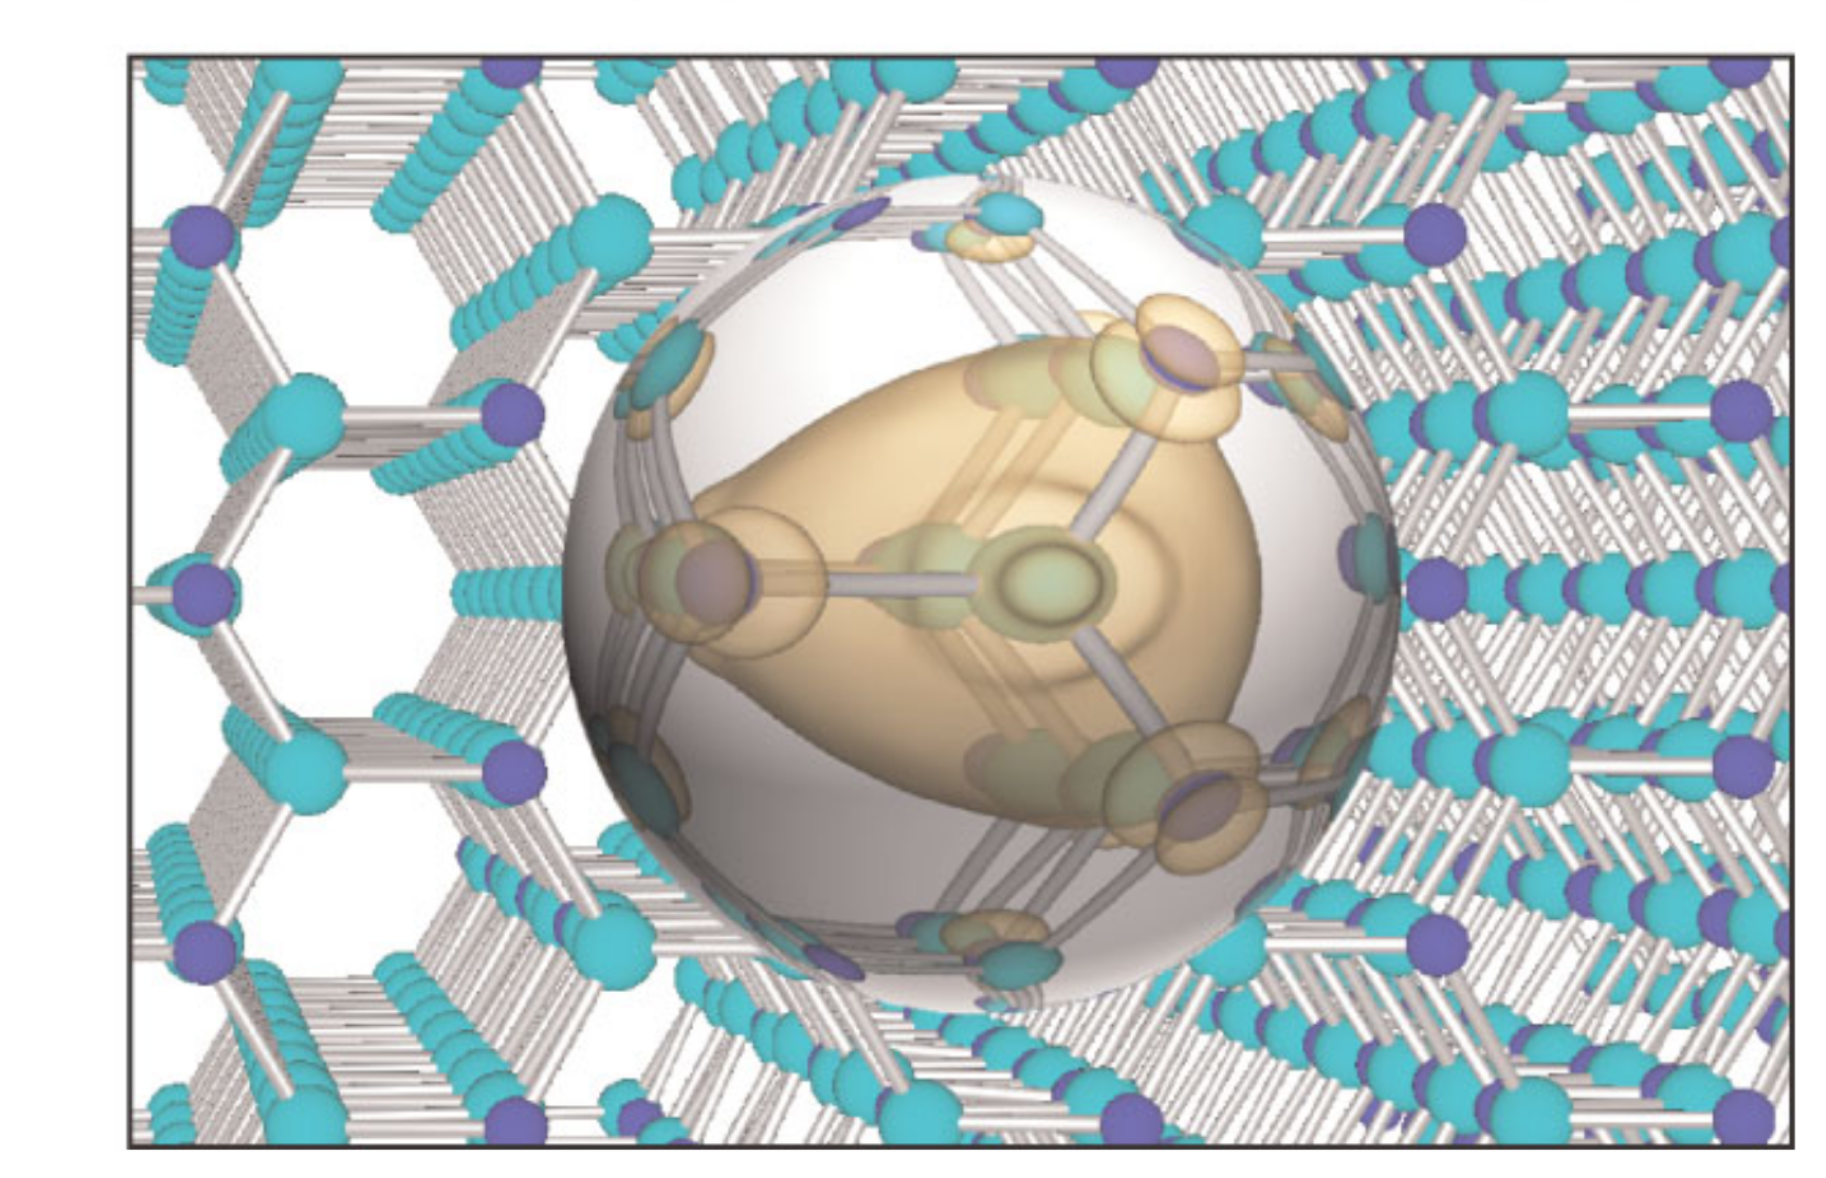
\includegraphics[width=0.5\linewidth]{lectures/figures/8_Defect_Charge_Density.png}
                \caption{Charge density of the $V_O^0$ gap state in ZnO. \cite{vandewalleAdvancesElectronicStructure2011}}
            \end{figure}

            \column{0.5\textwidth}
            \begin{figure}
                \centering
                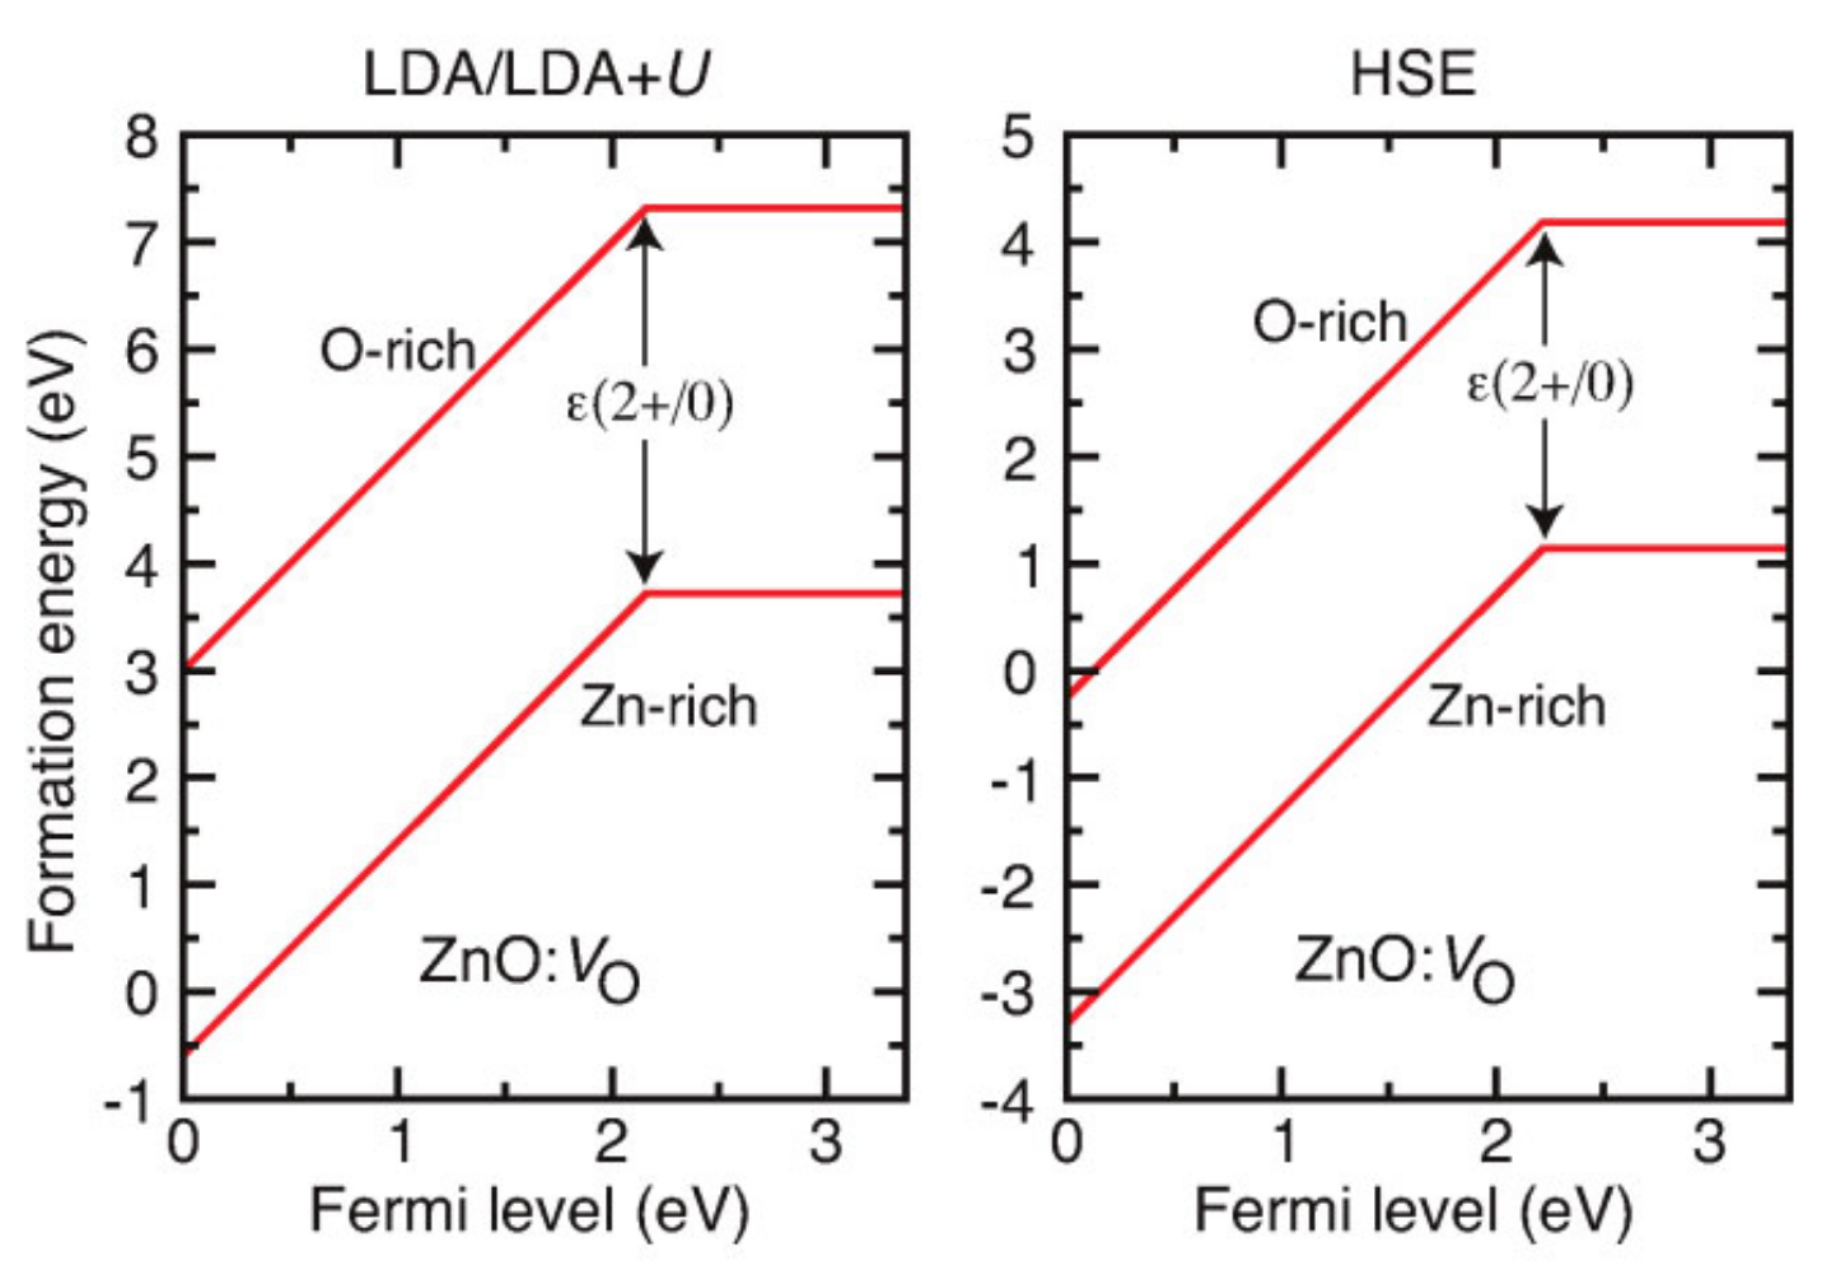
\includegraphics[width=0.85\linewidth]{lectures/figures/8_Defect_Diagram.png}
                \caption{Formation energy as a function of Fermi level for an oxygen vacancy (VO) in ZnO with (a) LDA/LDA+U and HSE.\cite{vandewalleAdvancesElectronicStructure2011}}
            \end{figure}

        \end{columns}

    \end{frame}

    \begin{frame}{Charged Defects}
        Coulomb interactions are strong and long-ranged
        \begin{itemize}
            \item True convergence wrt supercell size impractical.
            \item Extrapolation based on varying supercell sizes also typically computationally expensive.
            \item \textbf{General approach:} Relatively small supercells + correction scheme (Makov-Payne, Freysoldt, etc.).\cite{komsaComparisonVariousFinitesize2012}
        \end{itemize}

        \begin{equation*}
            E^f[X^q] = E_{total}[X^q] +\textcolor{red}{E^q_{corr}} - E^f[bulk] - \sum_i n_i \mu_i +\textcolor{red}{q[\varepsilon_f + \varepsilon_v +\Delta v_{o/b}]}
        \end{equation*}
        \begin{itemize}
            \item $E^q_{corr}$: Interaction between localized and background charge.
            \item $\varepsilon_f$: Fermi energy
            \item $\varepsilon_v$: Valence band maximum
            \item $\Delta v_{o/b}$: Alignment term for bulk vs defect supercells.
        \end{itemize}

    \end{frame}

    \begin{frame}{Example: Native defects in \ce{ZrO2} and \ce{HfO2}}

        \begin{columns}
            \column{0.5\textwidth}
            \begin{figure}
                \centering
                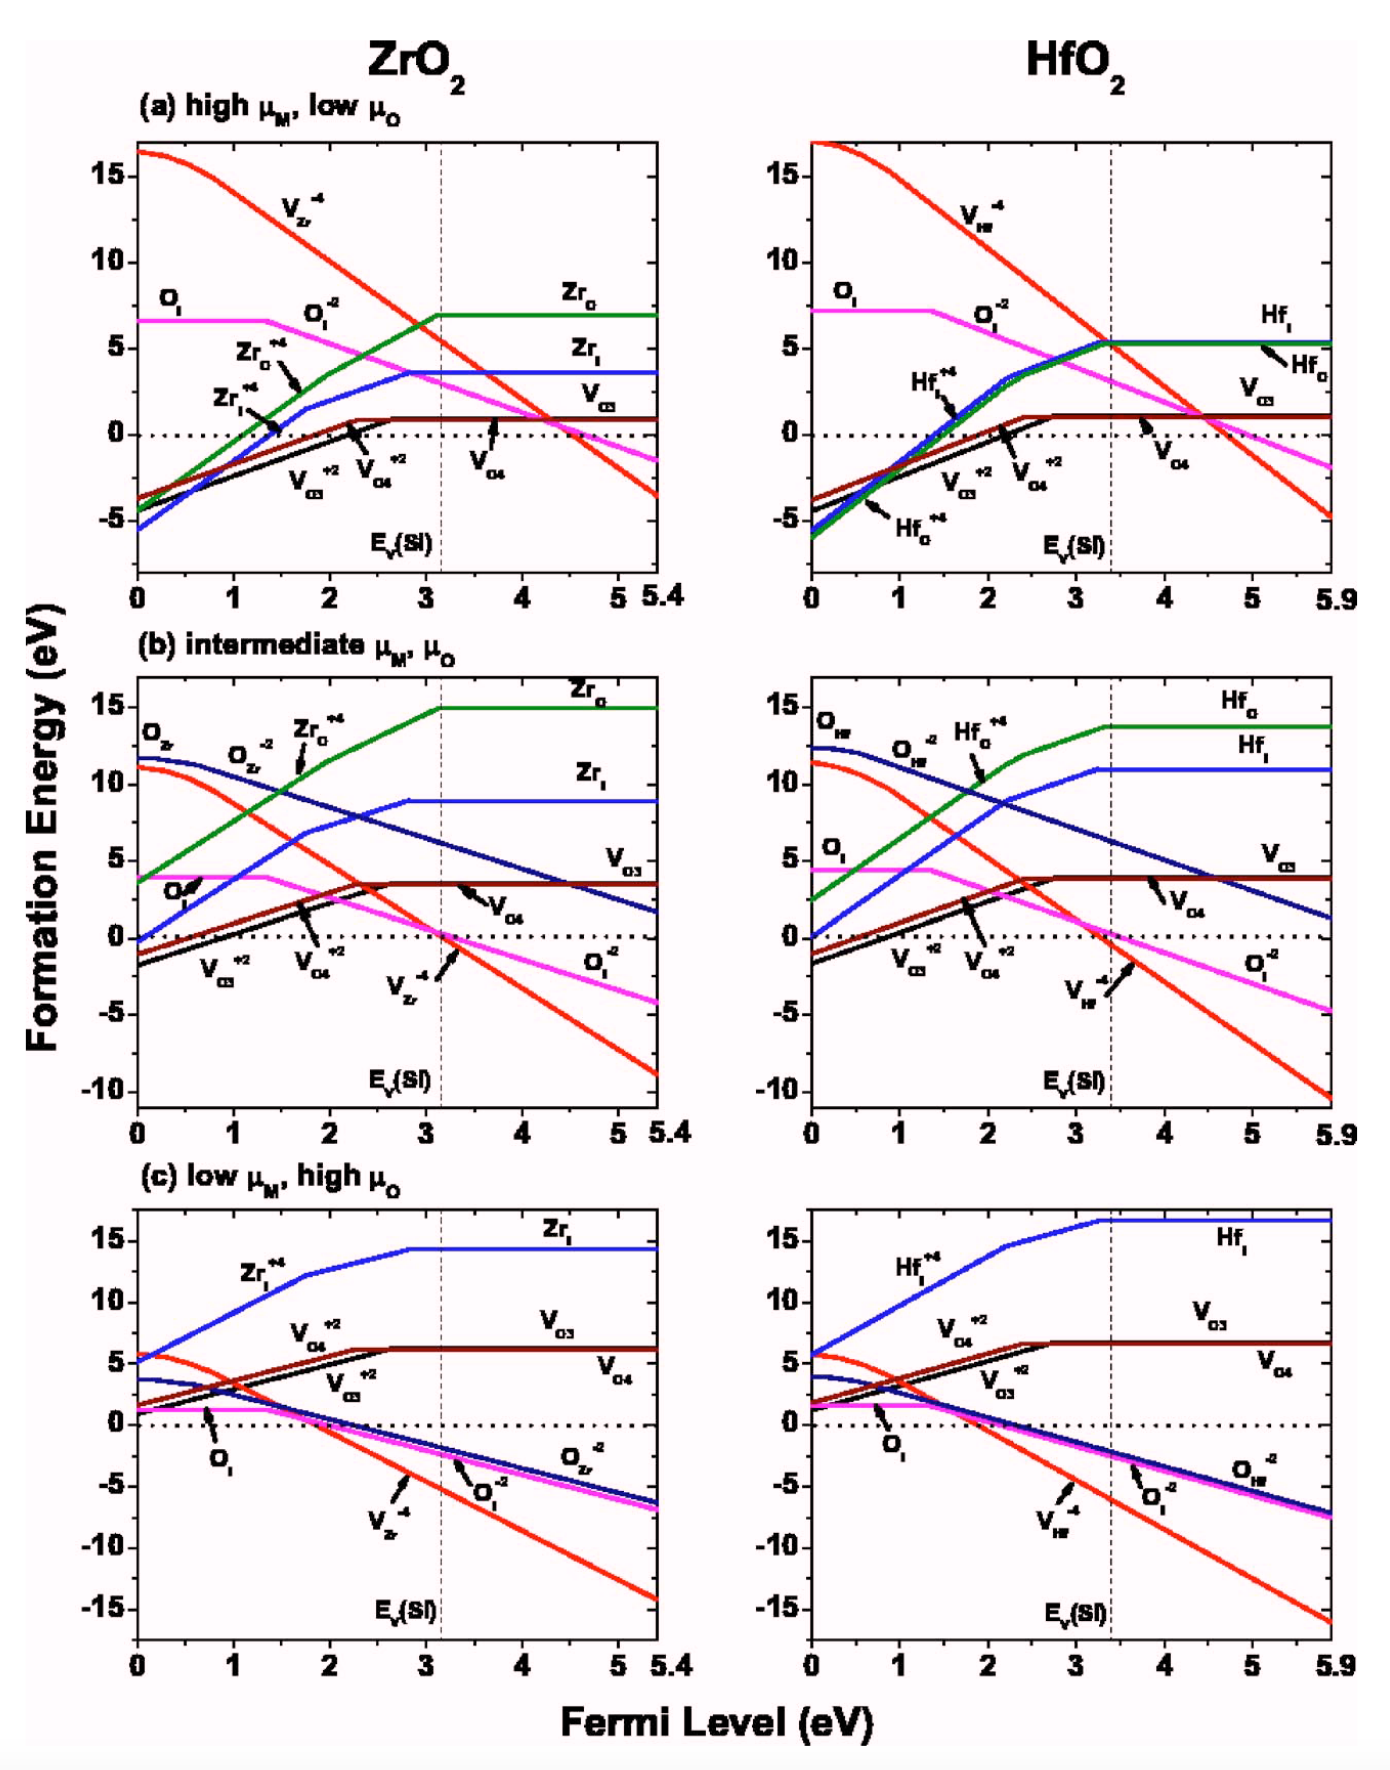
\includegraphics[width=0.7\linewidth]{lectures/figures/8_Defect_Diagram_ZrO2_HfO2.png}
            \end{figure}
            \column{0.5\textwidth}
            Calculated defect formation energy for native point defects in \ce{ZrO2} and \ce{HfO2} as a function of Fermi level and for (a)low oxygen partial pressure and high metal partial pressure, (b) intermediate oxygen and metal partial pressure, and (c) high oxygen partial pressure and low metal partial pressure.\cite{zhengFirstprinciplesStudyNative2007}
        \end{columns}

    \end{frame}

    \begin{frame}{Other topics}
        Phonons: To be covered in subsequent lectures on temperature.\newline
        \newline
        Surfaces and interfaces: An entire lecture by itself due to their importance in nanomaterials.


    \end{frame}

    \begin{frame}[allowframebreaks]{Bibliography}
        \bibliographystyle{unsrt}
        \bibliography{refs}
    \end{frame}



    \begin{frame}
        \Huge{\centerline{The End}}
    \end{frame}

\end{document}

